\newpage 
\subsection{DEIMOS}
DEIMOS determines the shape of objects using the second
order moments of the light profile as measured by and elliptical
Gaussian weight function. In this challenge the DEIMOS pipeline eliminates objects with $ \gamma > 1.0 $
from the catalog. \\
 
\begin{figure*}
\centering
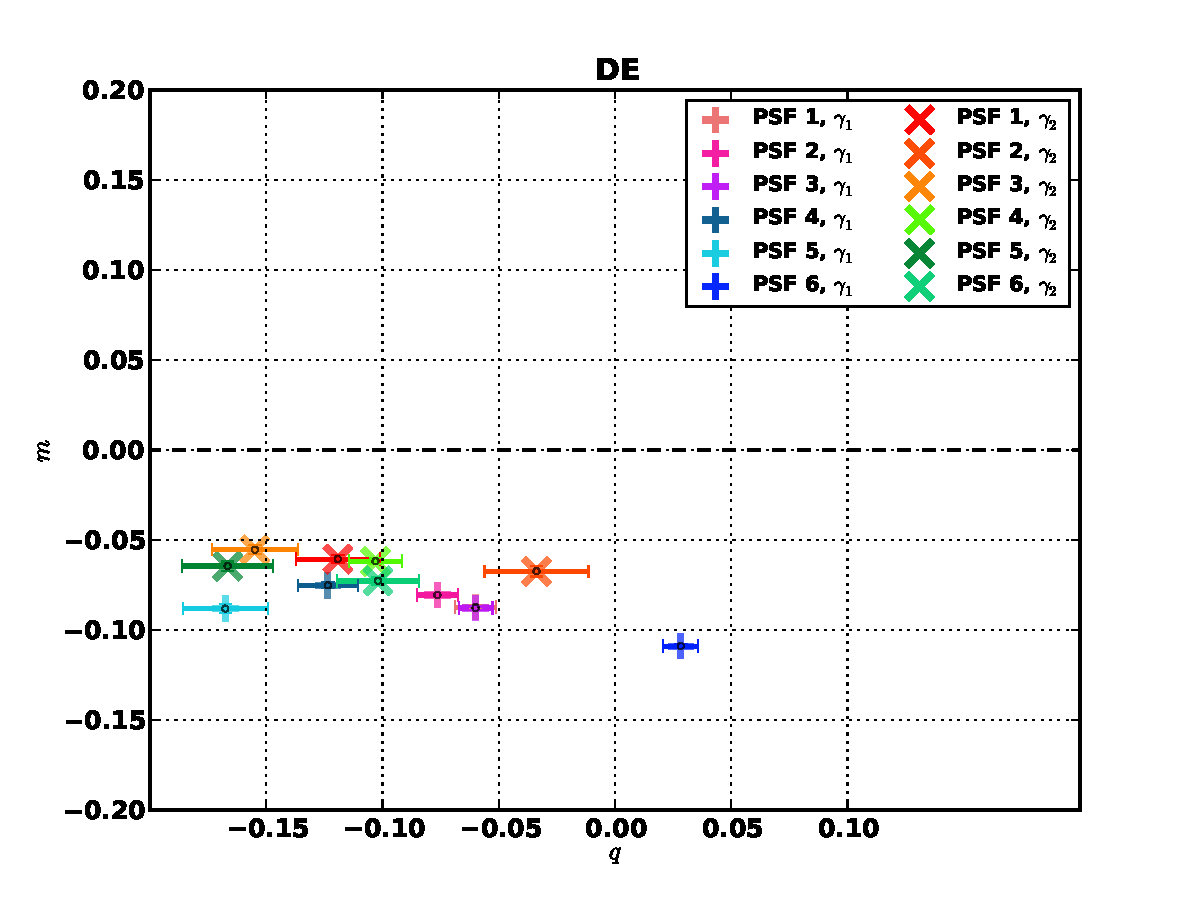
\includegraphics[width=0.45\textwidth]{fig/QMC_main_DE_f.pdf} 
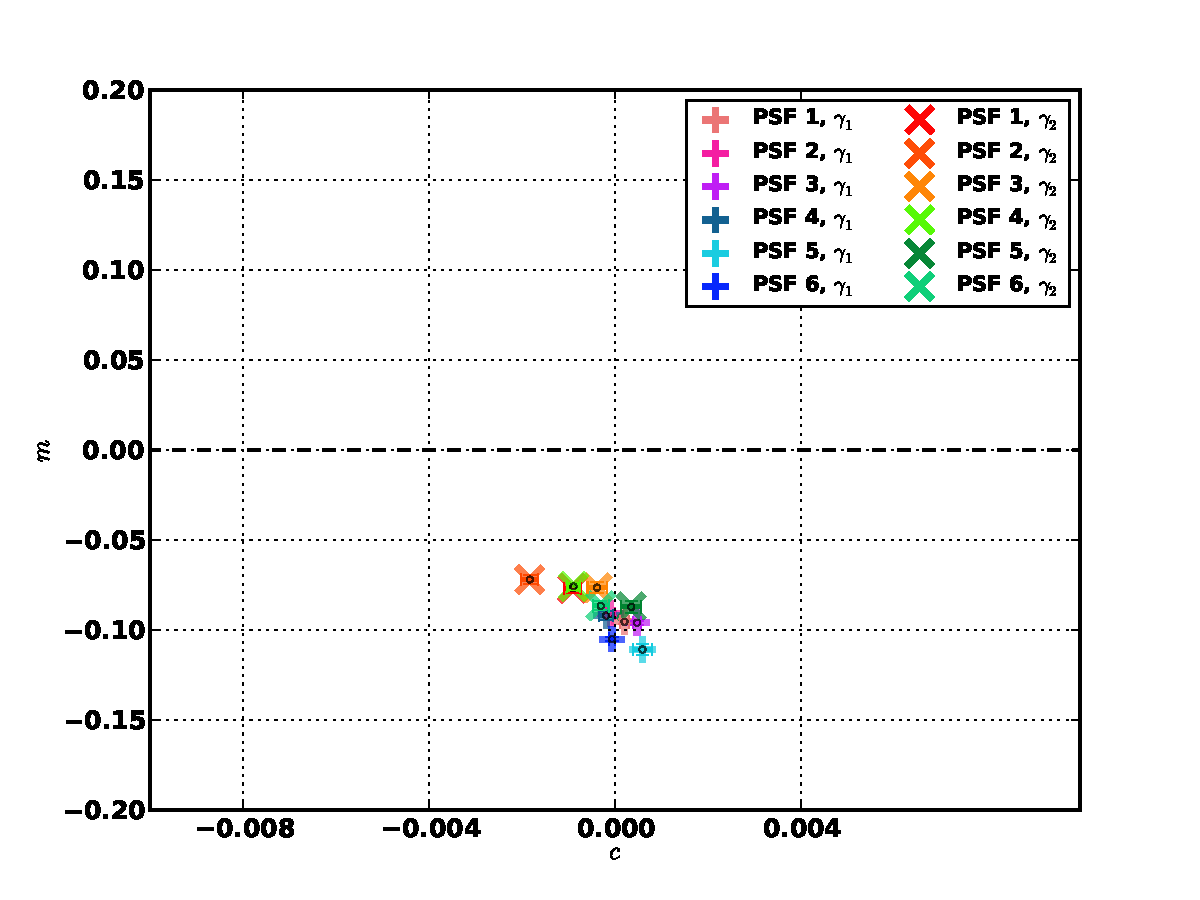
\includegraphics[width=0.45\textwidth]{fig/MC_main_DE_f.pdf} 
\caption{Average Q and M results for all pipelines for objects 
SNR $>$ 20 on the left and M and C results for all pipelines for objects 
SNR $>$ 20 on the right seperate by $\gamma_{1} $ and $\gamma_{2} $ as
well as PSF.}
\label{fig:DEIMOS_qmc}
\end{figure*}

\begin{figure*}
\centering
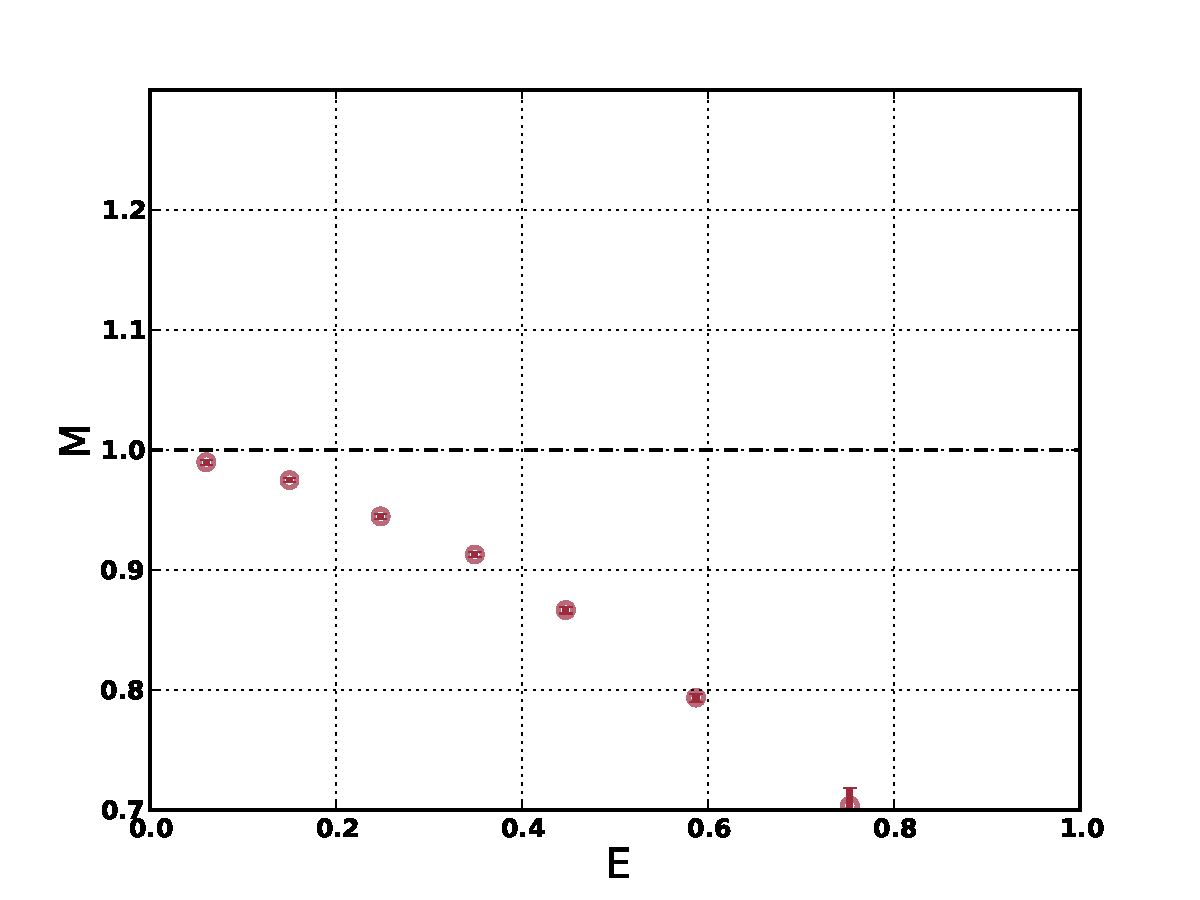
\includegraphics[width=0.45\textwidth]{fig/MvaleDE.pdf} 
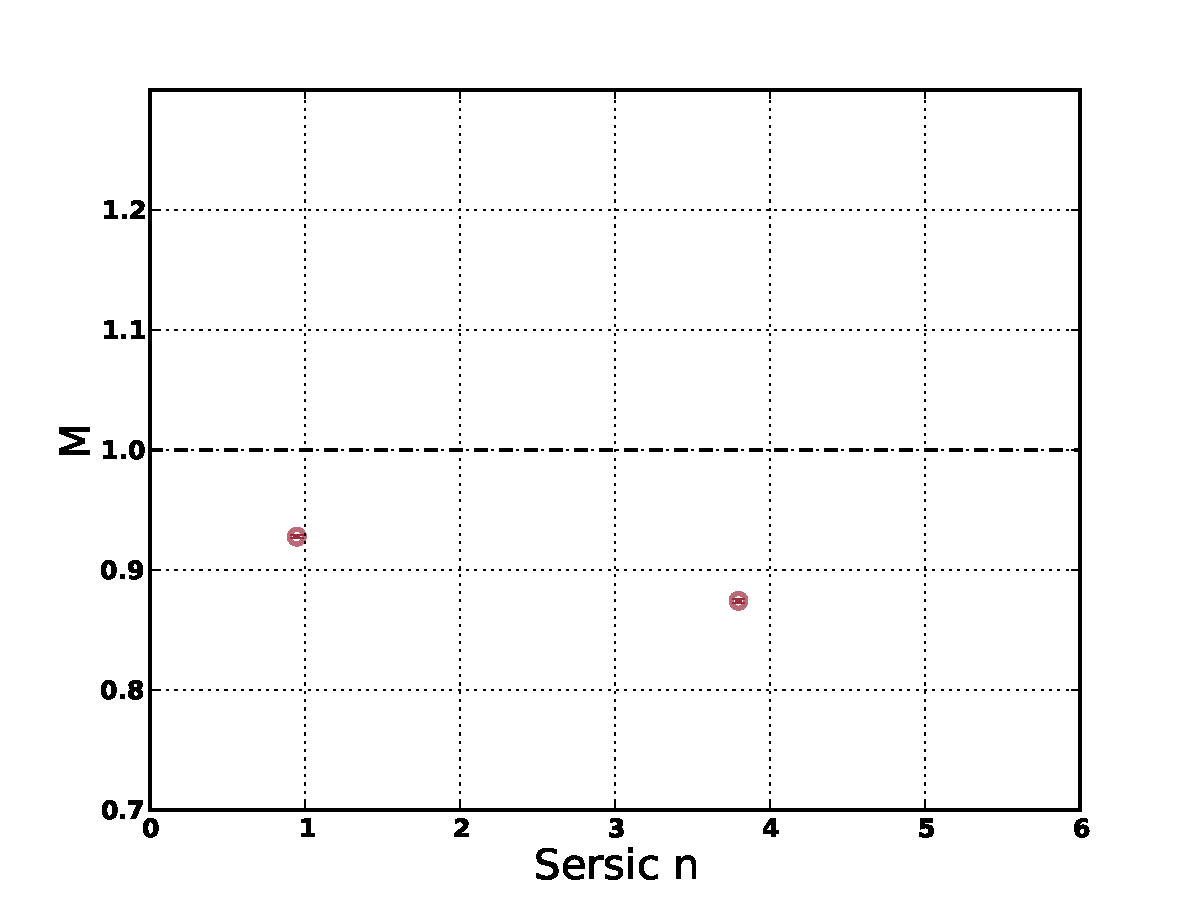
\includegraphics[width=0.45\textwidth]{fig/Mval_typeDE.pdf} 
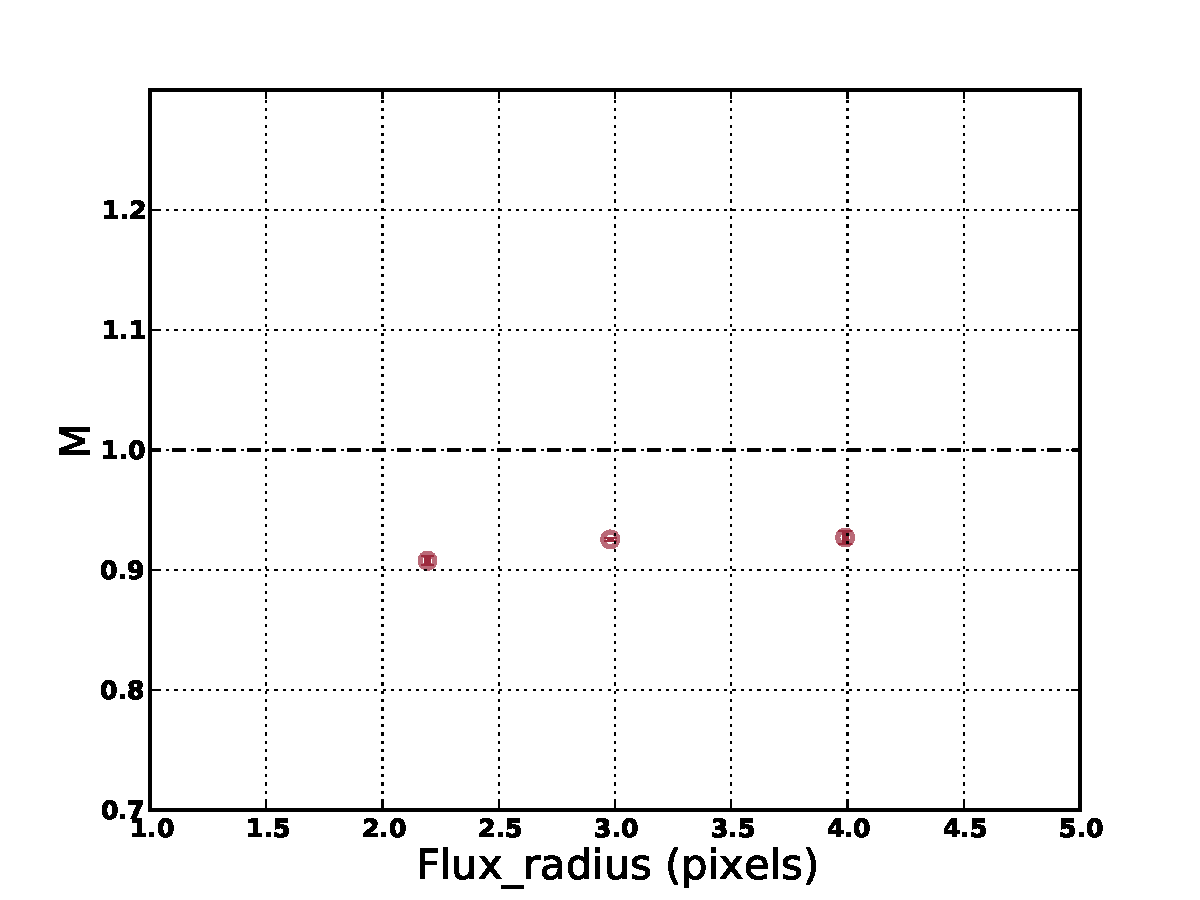
\includegraphics[width=0.45\textwidth]{fig/Mval_sizeDE.pdf} 
\caption{The M and C values for ...}
\label{fig:DEIMOS_m}
\end{figure*}

\newpage 
\subsection{IMCAT}
The KSB+ pipeline IMCAT measures the second order moments using an
elliptical gaussian. The implementation of IMCAT used on the CSTEP images
took an average of the $P^{sm}$ and $p^*$ of selected stars in the
image to calculate the PSF. The average of the trace of the two
matrices $P^{sm}$ and $P^{sh}$ were multiplied by the identity
matrix. The IMCAT pipeline eliminates objects with $ \gamma > 1.0 $
from the catalog.  \\

\begin{figure*}
\centering
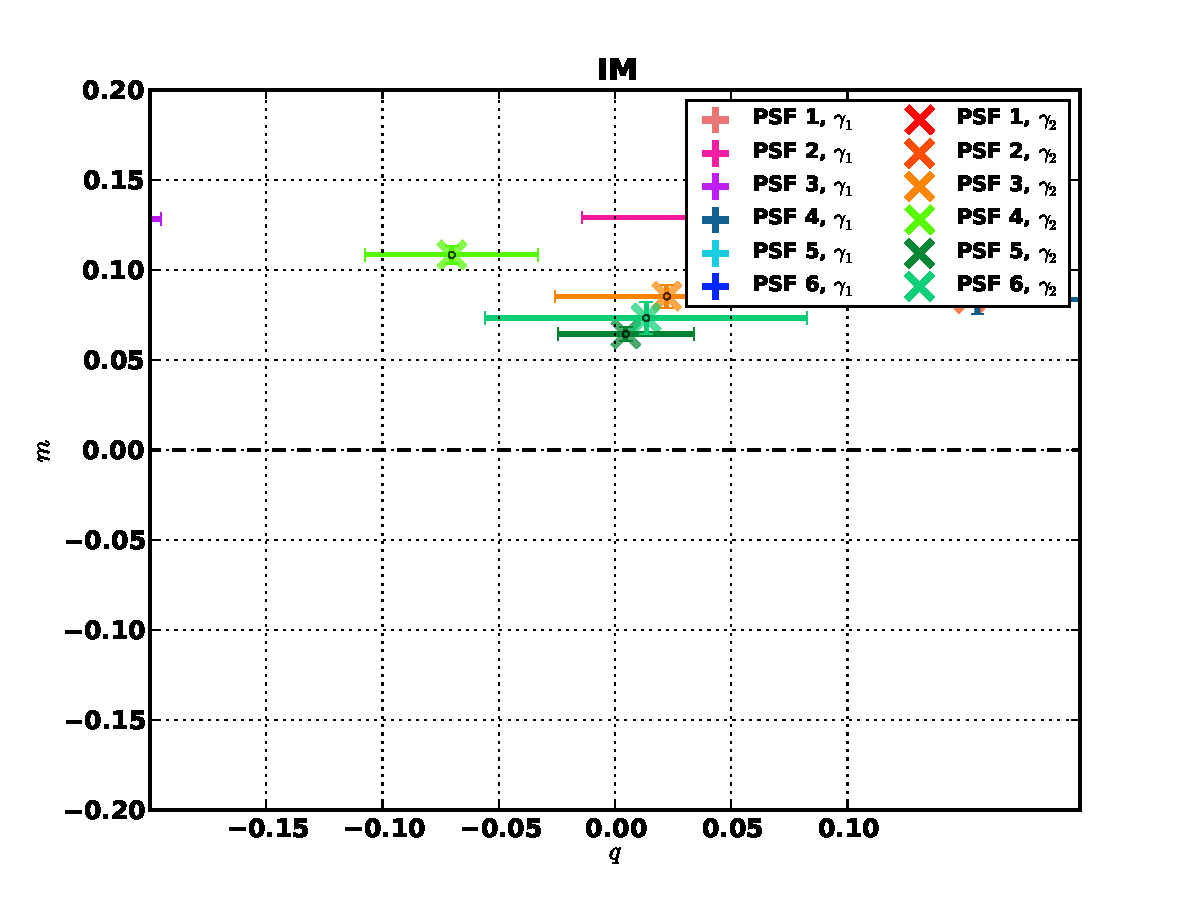
\includegraphics[width=0.45\textwidth]{fig/QMC_main_IM_f.pdf} 
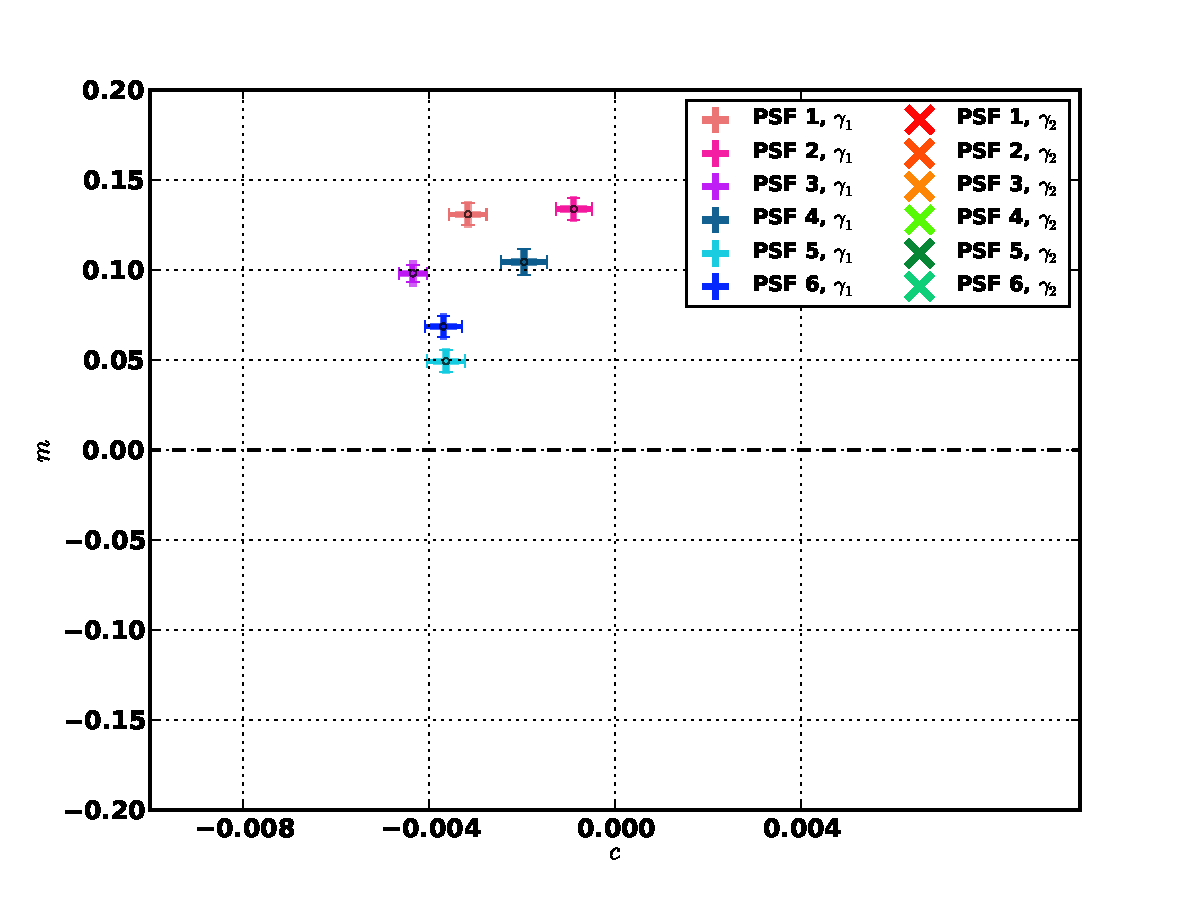
\includegraphics[width=0.45\textwidth]{fig/MC_main_IM_f.pdf} 
\caption{Average Q and M results for all pipelines for objects 
SNR $>$ 20 on the left and M and C results for all pipelines for objects 
SNR $>$ 20 on the right seperate by $\gamma_{1} $ and $\gamma_{2} $ as
well as PSF.}
\label{fig:IMCAT_qmc}
\end{figure*}

\begin{figure*}
\centering
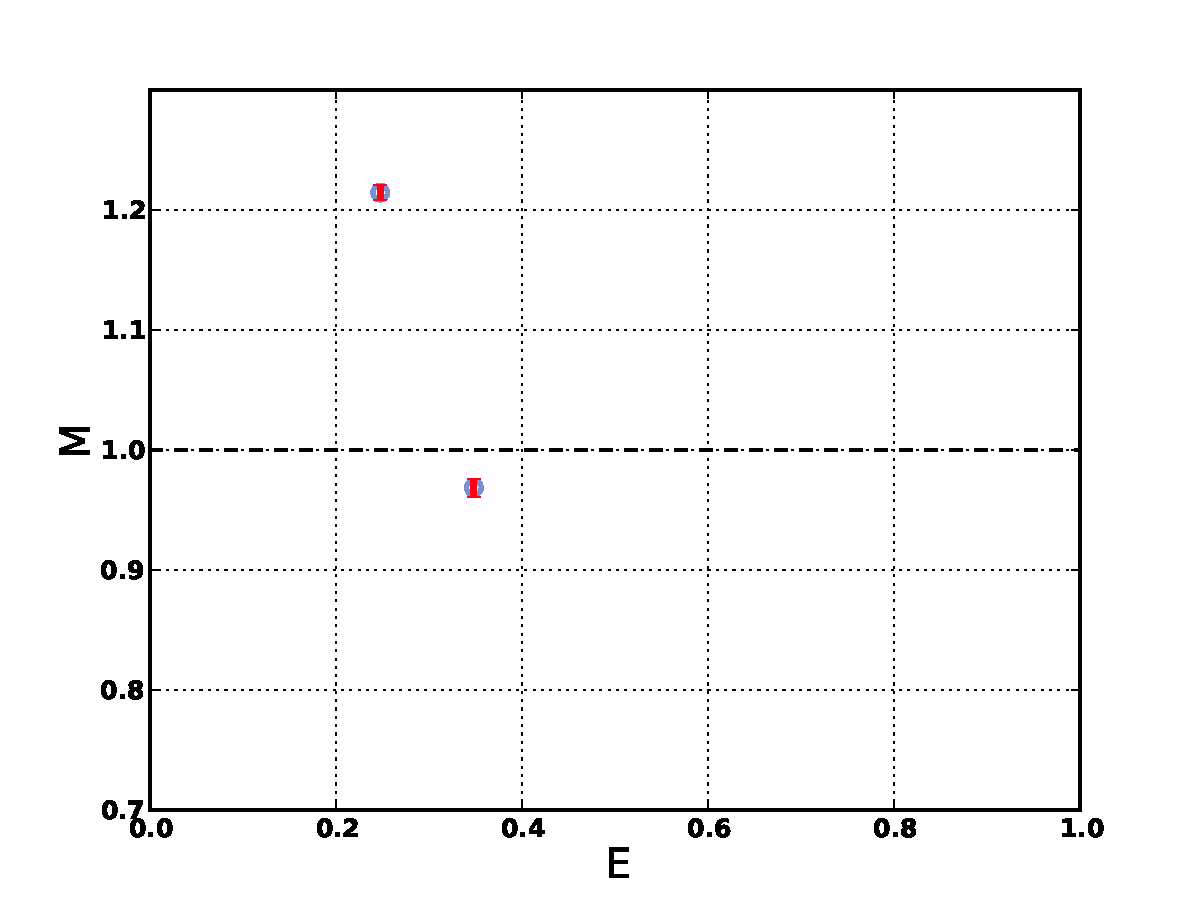
\includegraphics[width=0.45\textwidth]{fig/MvaleIM.pdf} 
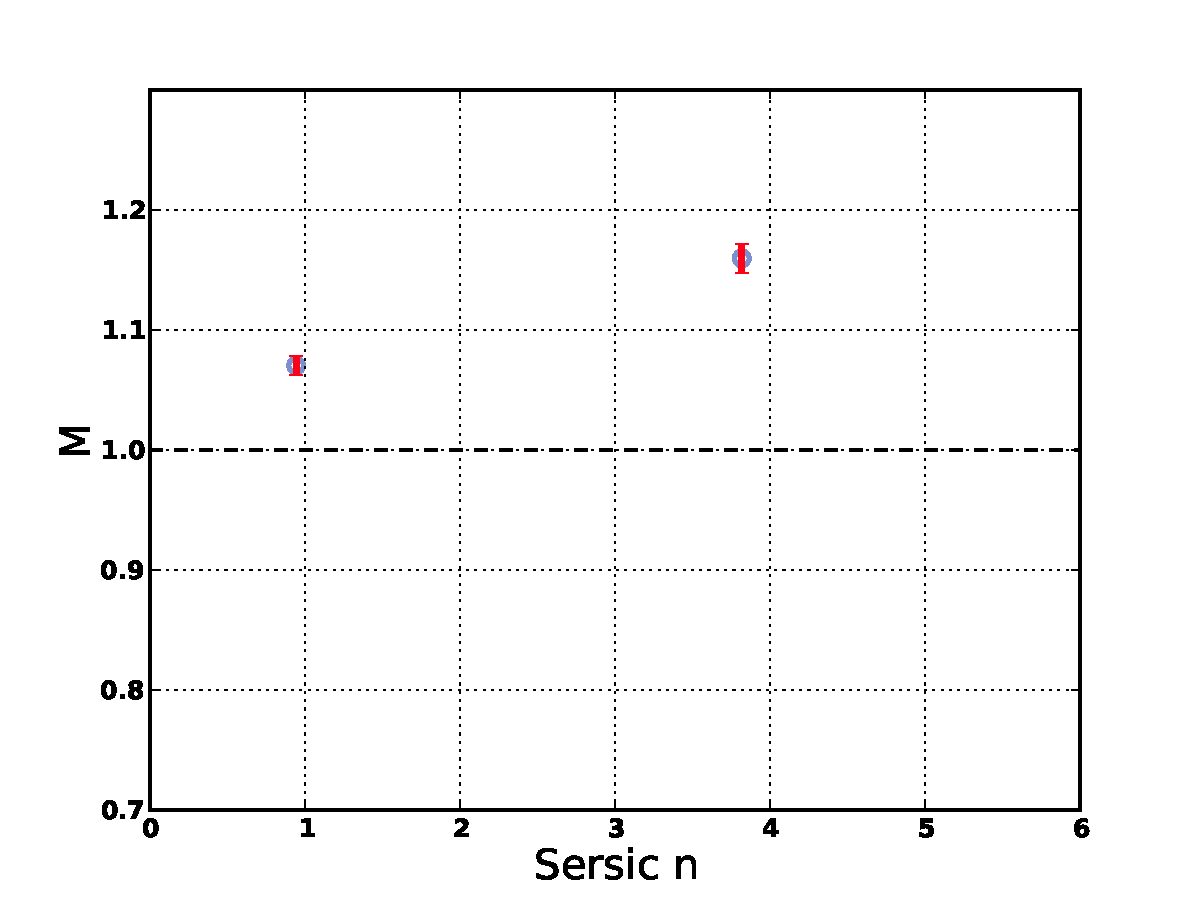
\includegraphics[width=0.45\textwidth]{fig/Mval_typeIM.pdf} 
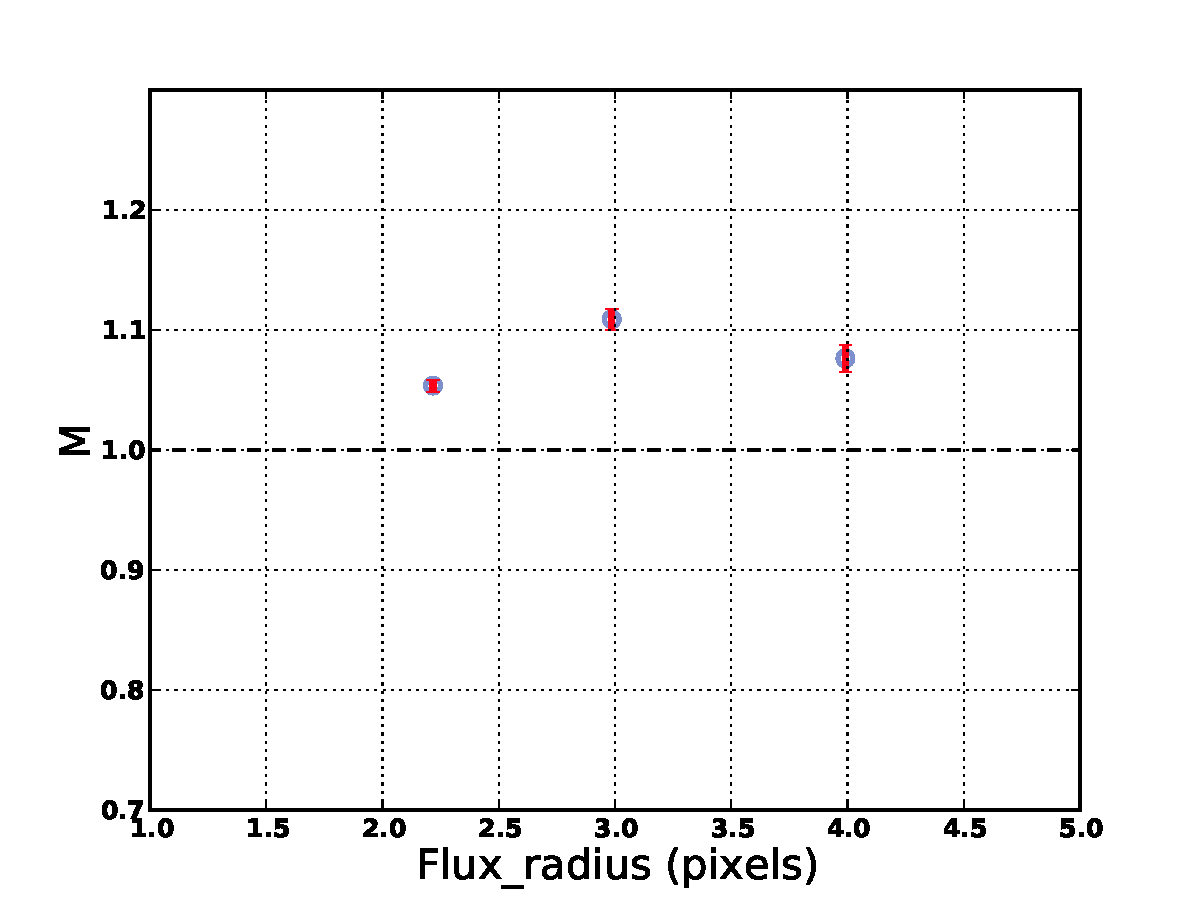
\includegraphics[width=0.45\textwidth]{fig/Mval_sizeIM.pdf} 
\caption{The M and C values for ...}
\label{fig:DEIMOS_m}
\end{figure*}

\newpage 
\subsection{ksbm}
The ksbm pipeline version used here is the same as the version
used to analyze the image sinulations in the GREAT10 challenge. This
KSB+ implementation uses elements of the 
DEMIOS lensing pipeline to determine the galaxy centroid and the
optimal size of the weighting function. There are no correction
factors applied, but objects with $\gamma > 1.0 $ are eliminated from
the final catalog. \\

\begin{figure*}
\centering
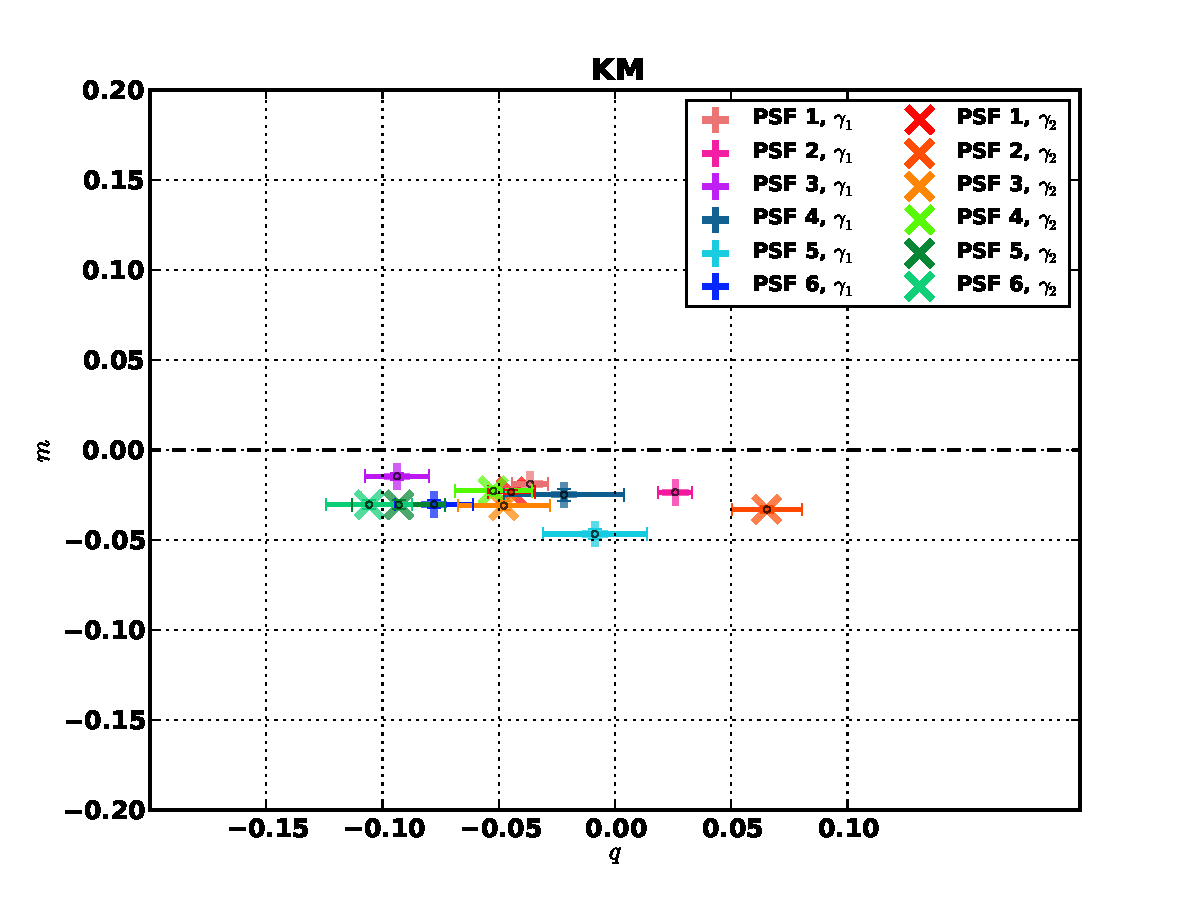
\includegraphics[width=0.45\textwidth]{fig/QMC_main_KM_f.pdf} 
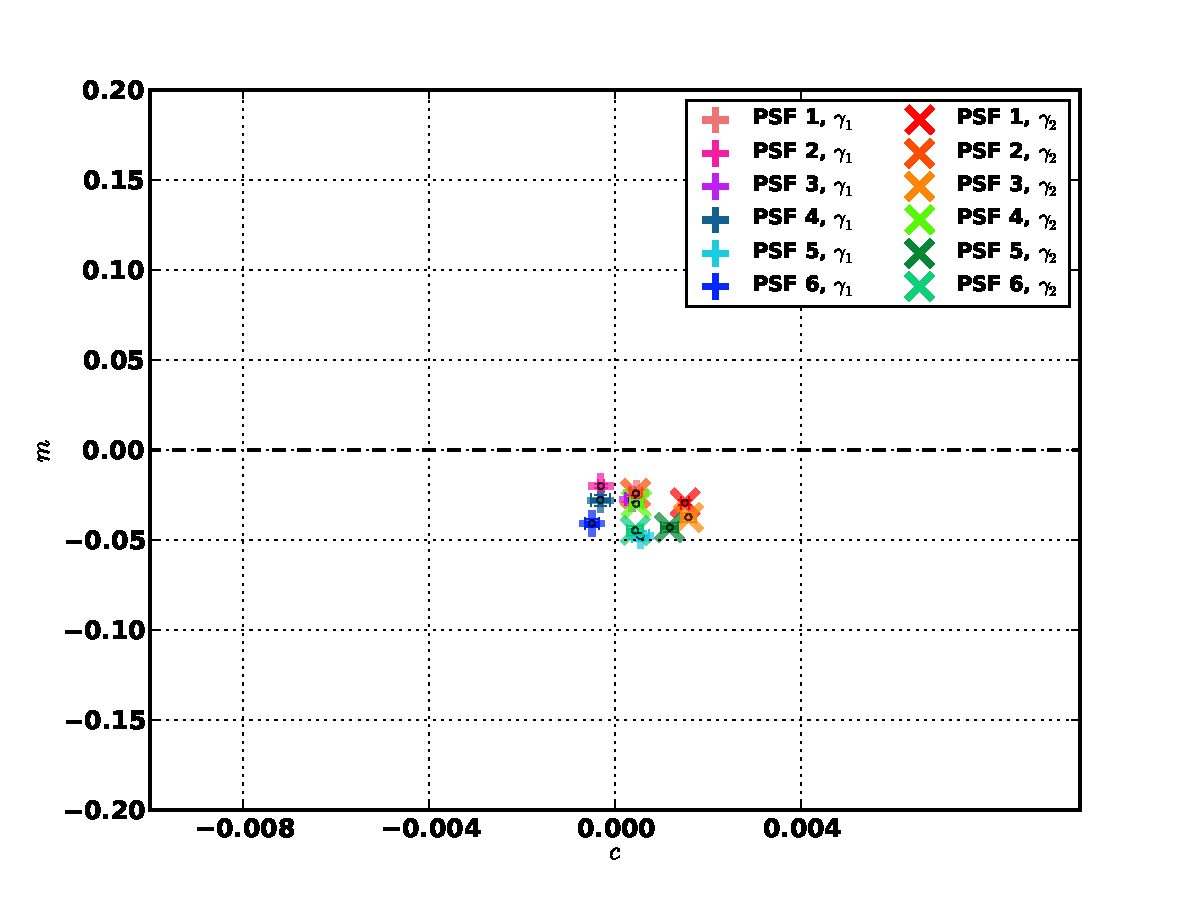
\includegraphics[width=0.45\textwidth]{fig/MC_main_KM_f.pdf} 
\caption{Average Q and M results for all pipelines for objects 
SNR $>$ 20 on the left and M and C results for all pipelines for objects 
SNR $>$ 20 on the right seperate by $\gamma_{1} $ and $\gamma_{2} $ as
well as PSF.}
\label{fig:ksbm_qmc}
\end{figure*}

\begin{figure*}
\centering
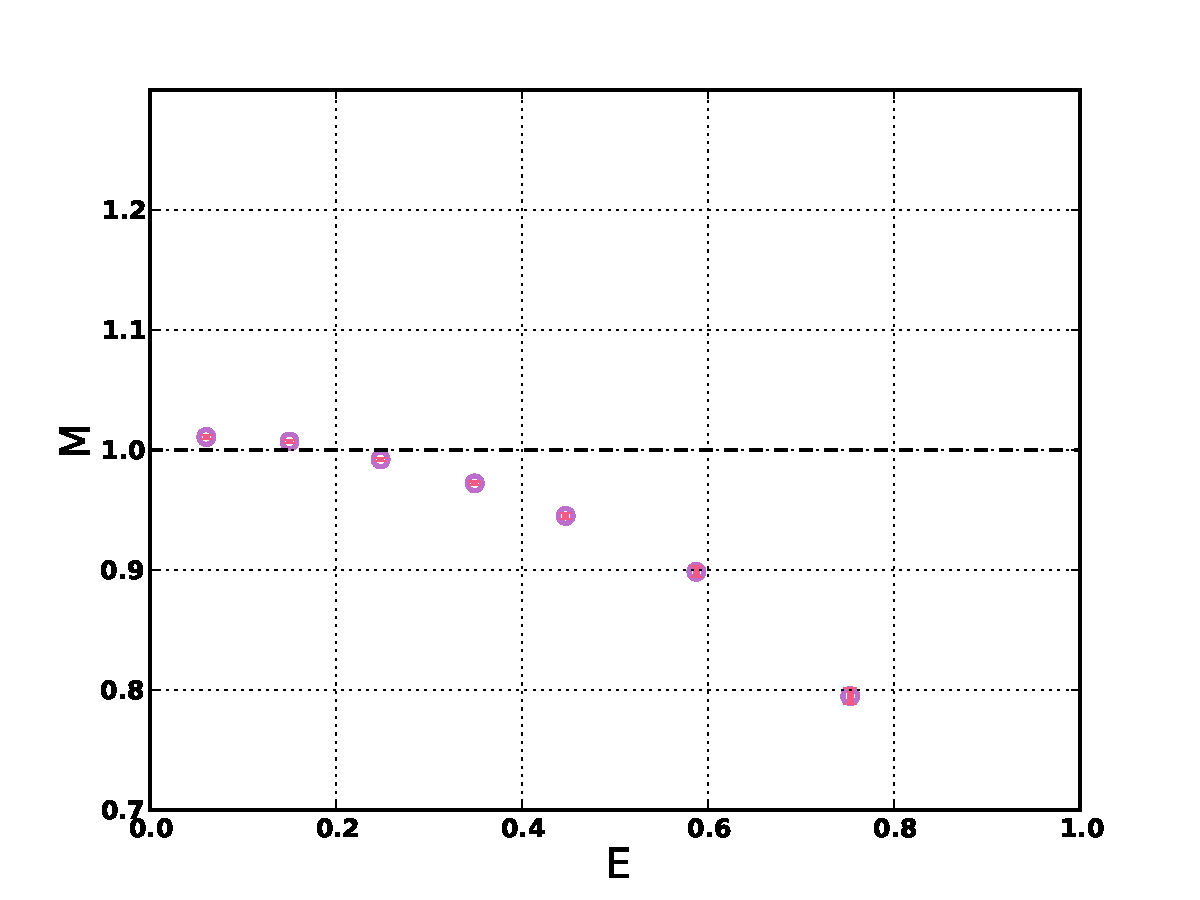
\includegraphics[width=0.45\textwidth]{fig/MvaleKM.pdf} 
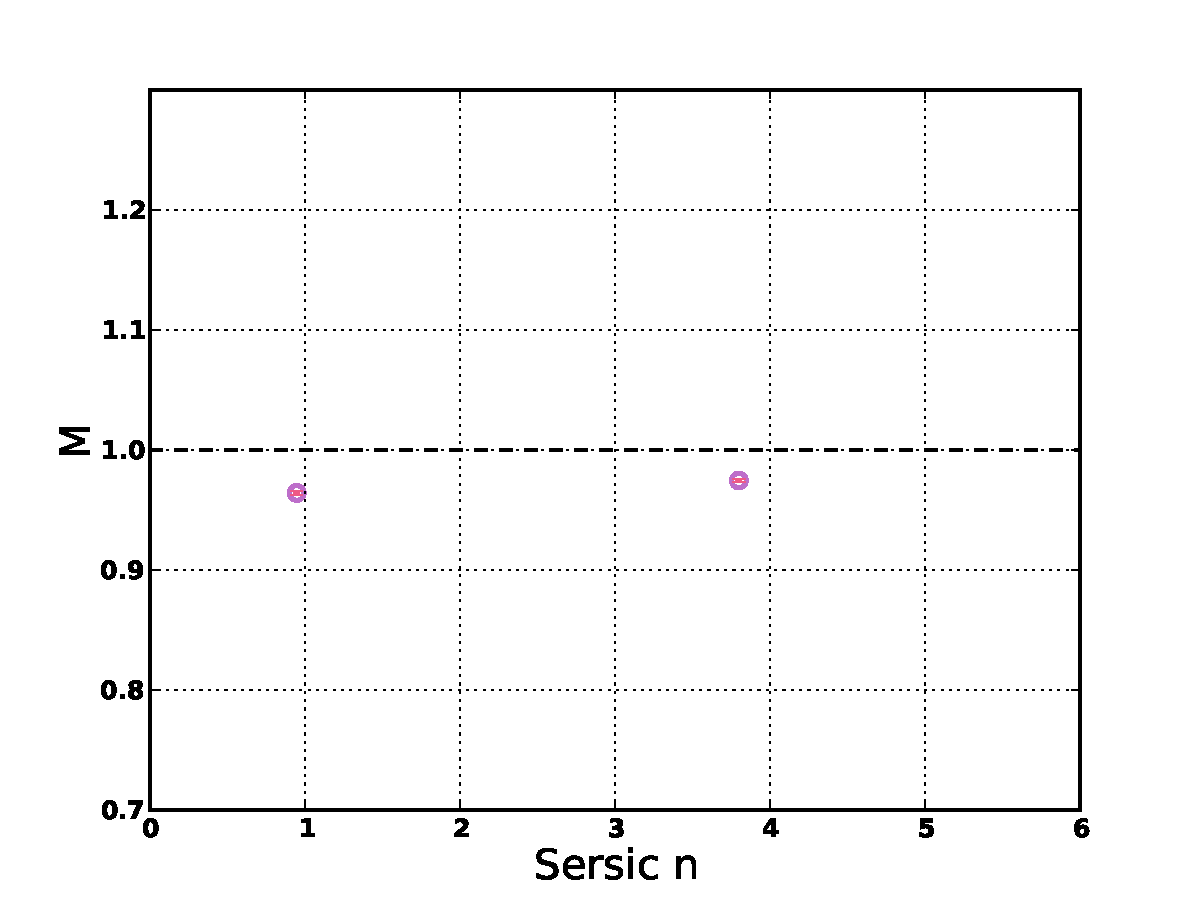
\includegraphics[width=0.45\textwidth]{fig/Mval_typeKM.pdf} 
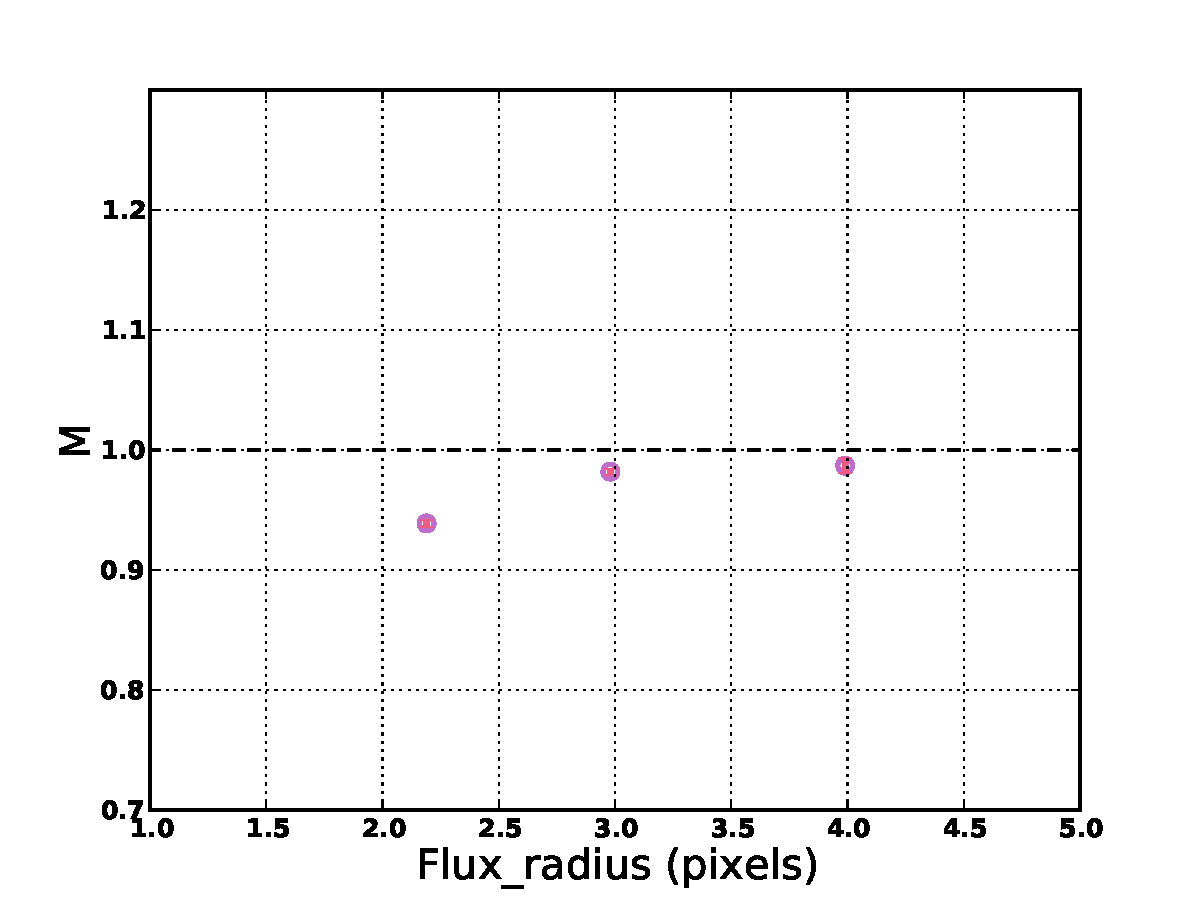
\includegraphics[width=0.45\textwidth]{fig/Mval_sizeKM.pdf} 
\caption{The M and C values for ...}
\label{fig:DEIMOS_m}
\end{figure*}

\newpage 
\subsection{PKSB}
PKSB is a lensing pipeline that uses the PSFEx \cite{PSFex}
to create a model of the PSF and an implementation of KSB+ method 
for shape measurement. A modified version of this lensing pipeline
that incorperates correction of shape measurement bias, based on the
CSTEP simulations, has been used to measure the mass of galaxy
clusters in \cite{Gruen_s} and \cite{Gruen2}. \\
 
\begin{figure*}
\centering
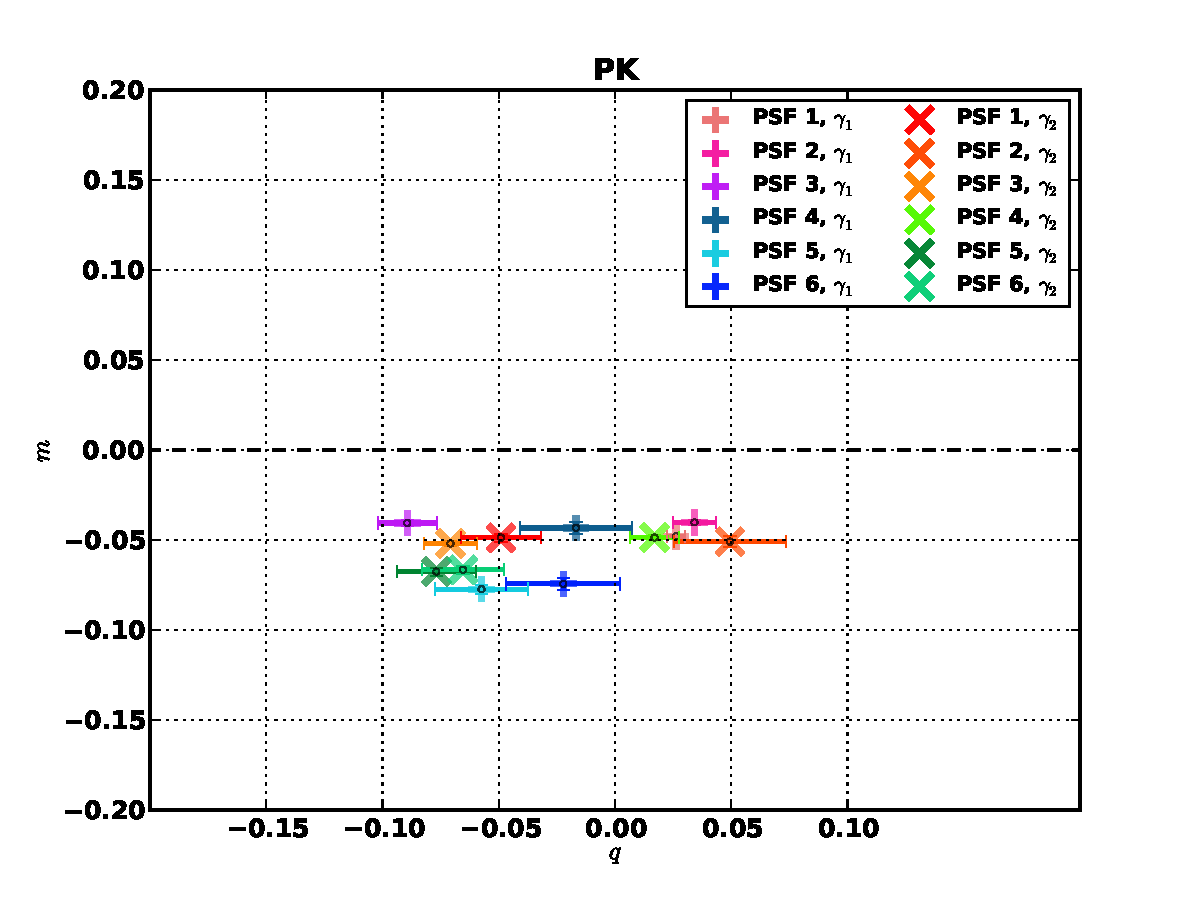
\includegraphics[width=0.45\textwidth]{fig/QMC_main_PK_f.pdf} 
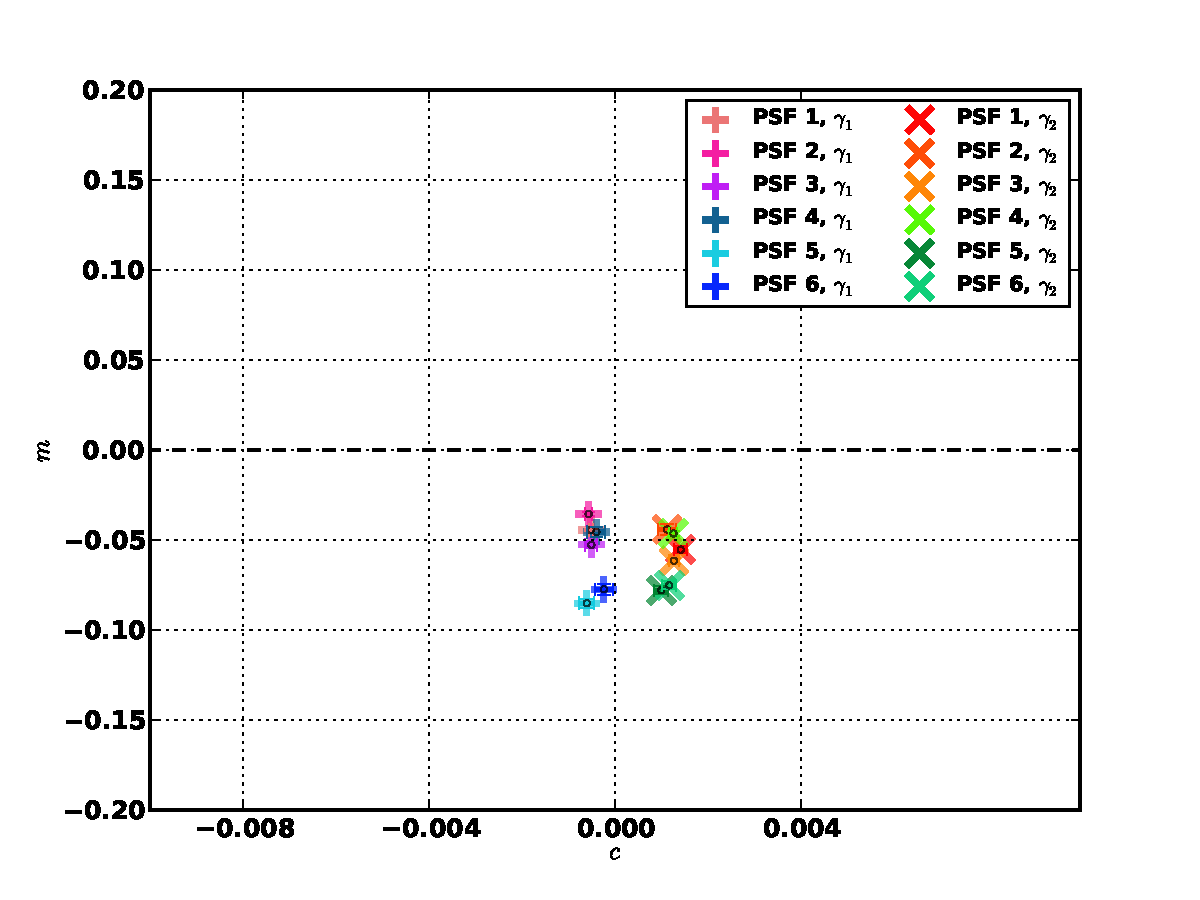
\includegraphics[width=0.45\textwidth]{fig/MC_main_PK_f.pdf} 
\caption{Average Q and M results for all pipelines for objects 
SNR $>$ 20 on the left and M and C results for all pipelines for objects 
SNR $>$ 20 on the right seperate by $\gamma_{1} $ and $\gamma_{2} $ as
well as PSF.}
\label{fig:PKSB_qmc}
\end{figure*}

\begin{figure*}
\centering
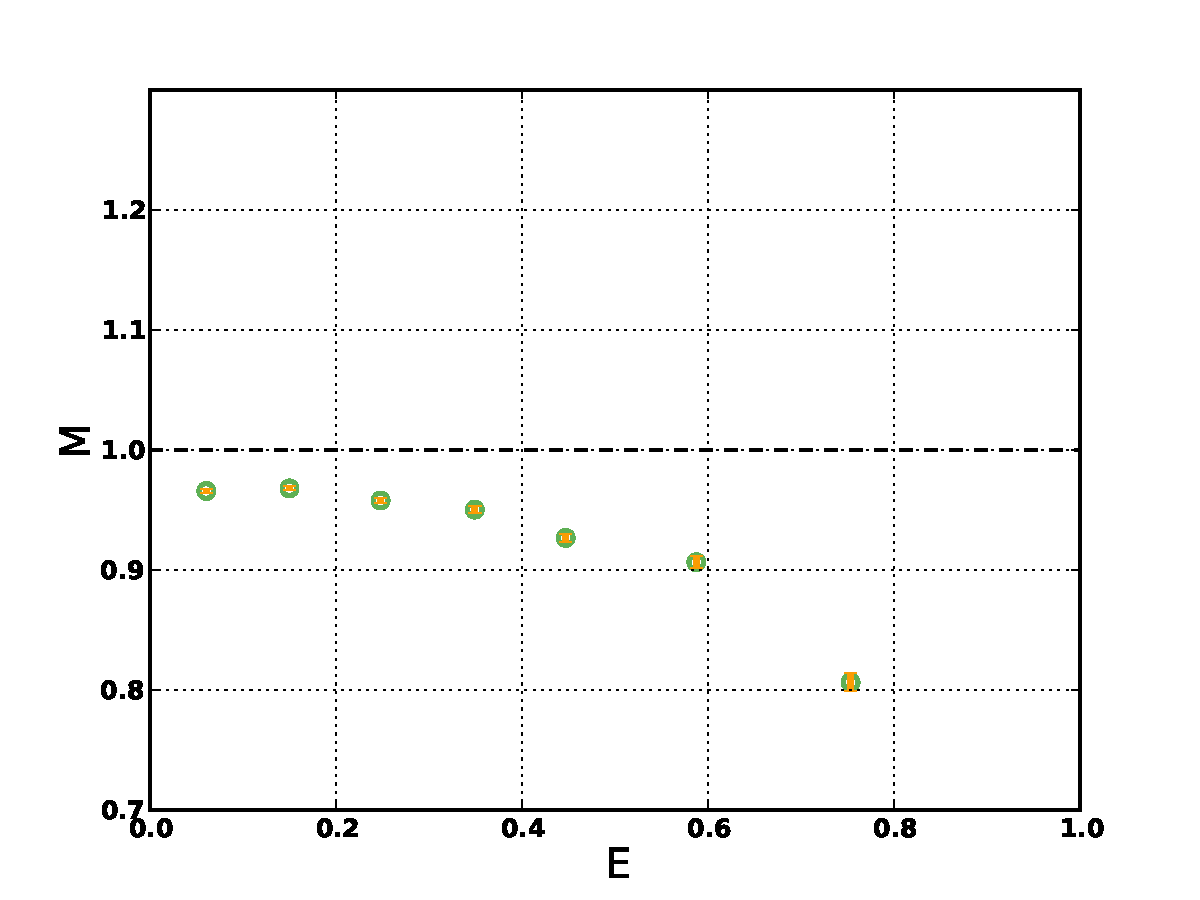
\includegraphics[width=0.45\textwidth]{fig/MvalePK.pdf} 
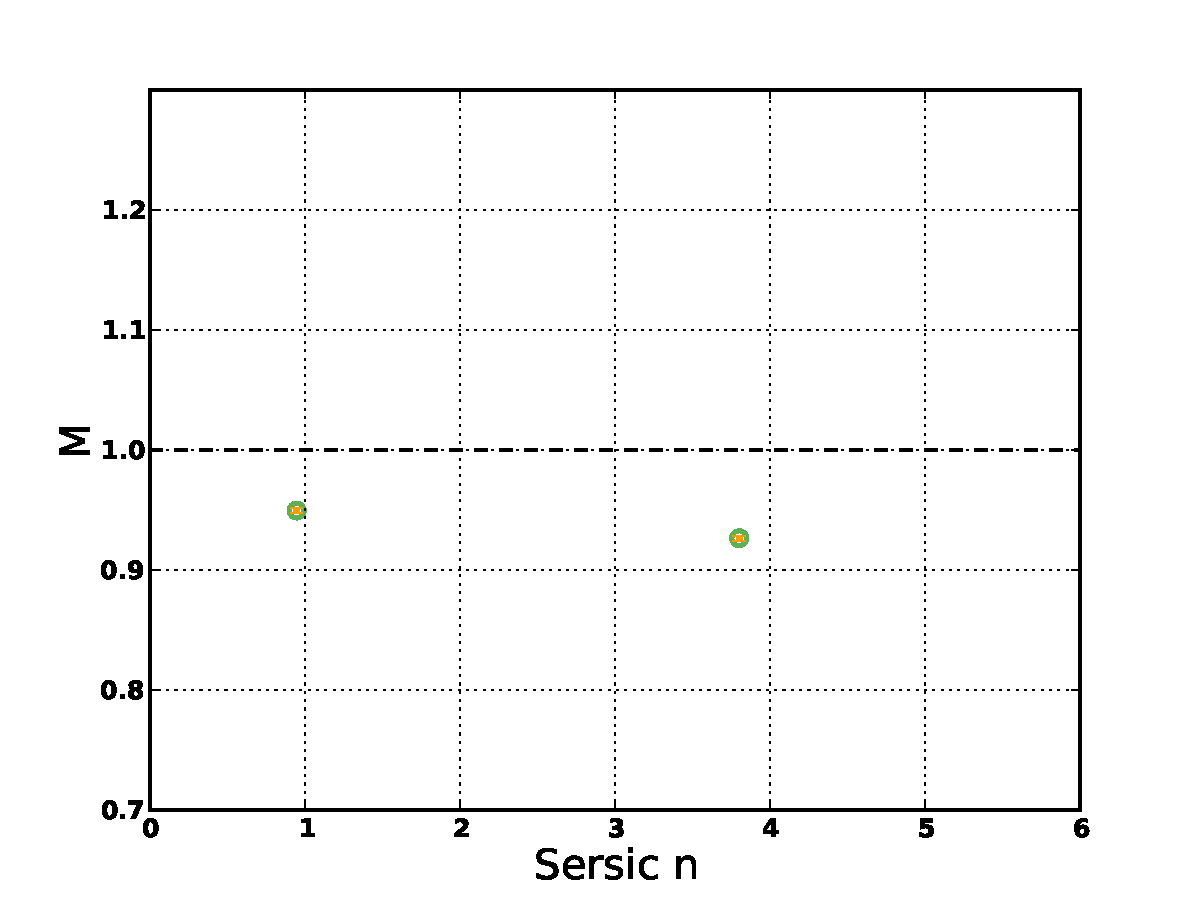
\includegraphics[width=0.45\textwidth]{fig/Mval_typePK.pdf} 
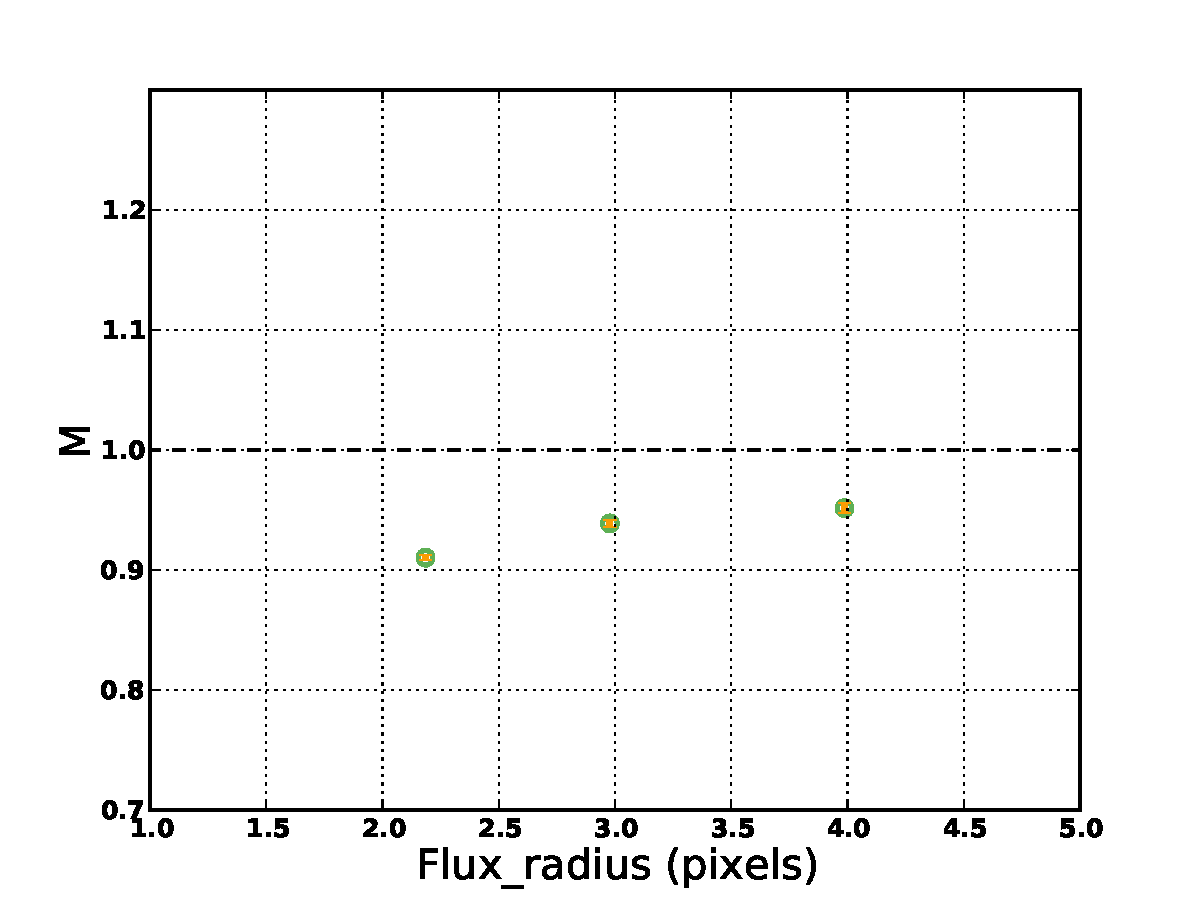
\includegraphics[width=0.45\textwidth]{fig/Mval_sizePK.pdf} 
\caption{The M and C values for ...}
\label{fig:DEIMOS_m}
\end{figure*}

\newpage 
\subsection{Gaussian Mixtures}
\begin{figure*}
\centering
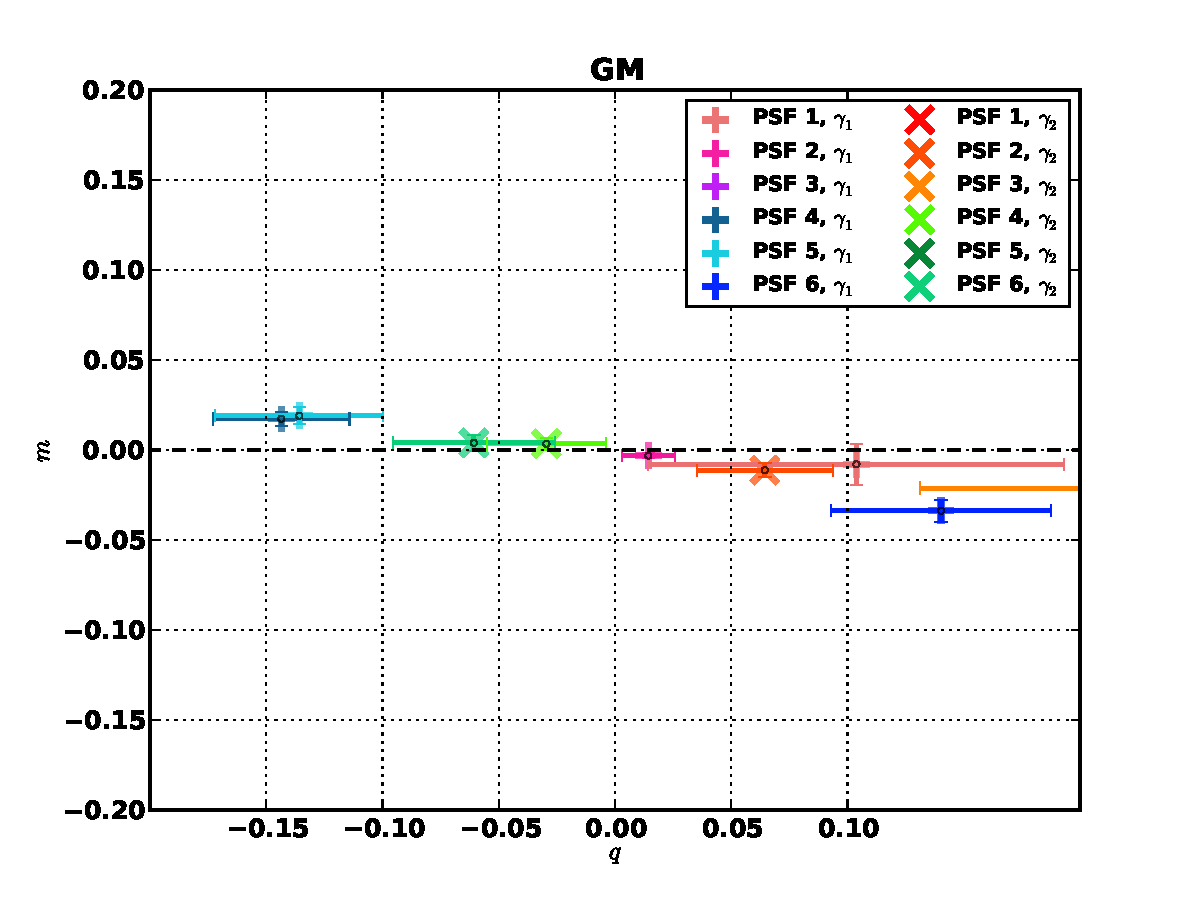
\includegraphics[width=0.45\textwidth]{fig/QMC_main_GM_f.pdf} 
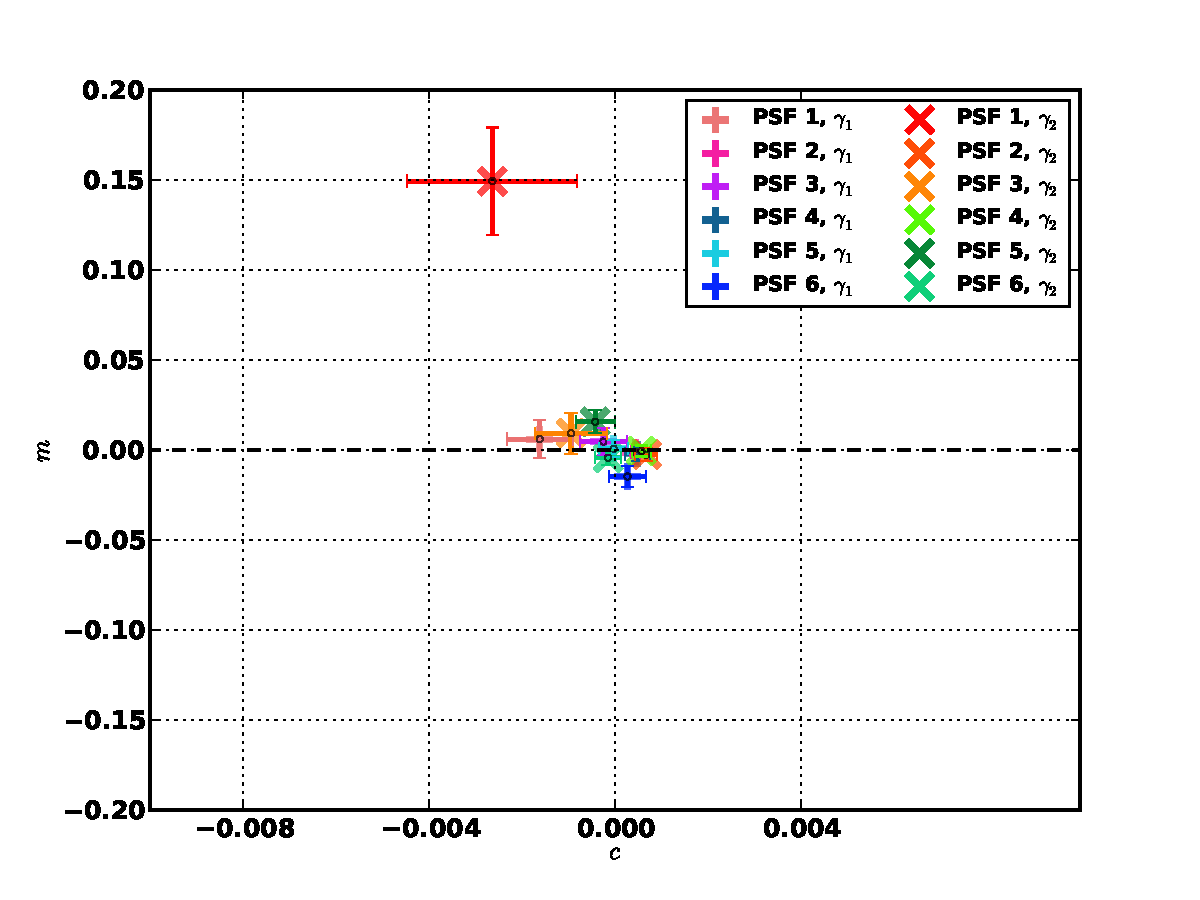
\includegraphics[width=0.45\textwidth]{fig/MC_main_GM_f.pdf} 
\caption{Average Q and M results for all pipelines for objects 
SNR $>$ 20 on the left and M and C results for all pipelines for objects 
SNR $>$ 20 on the right seperate by $\gamma_{1} $ and $\gamma_{2} $ as
well as PSF.}
\label{fig:Gmix_qmc}
\end{figure*}

\begin{figure*}
\centering
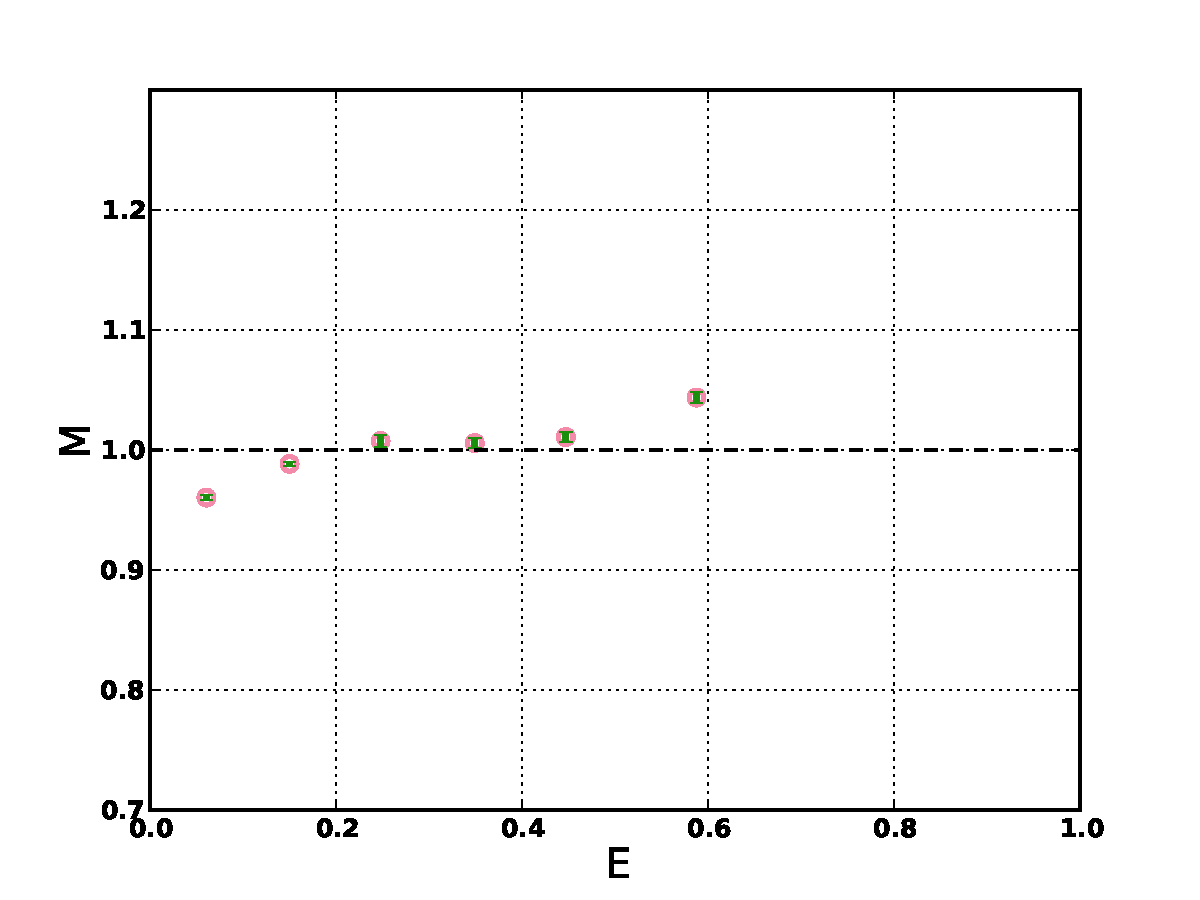
\includegraphics[width=0.45\textwidth]{fig/MvaleGM.pdf} 
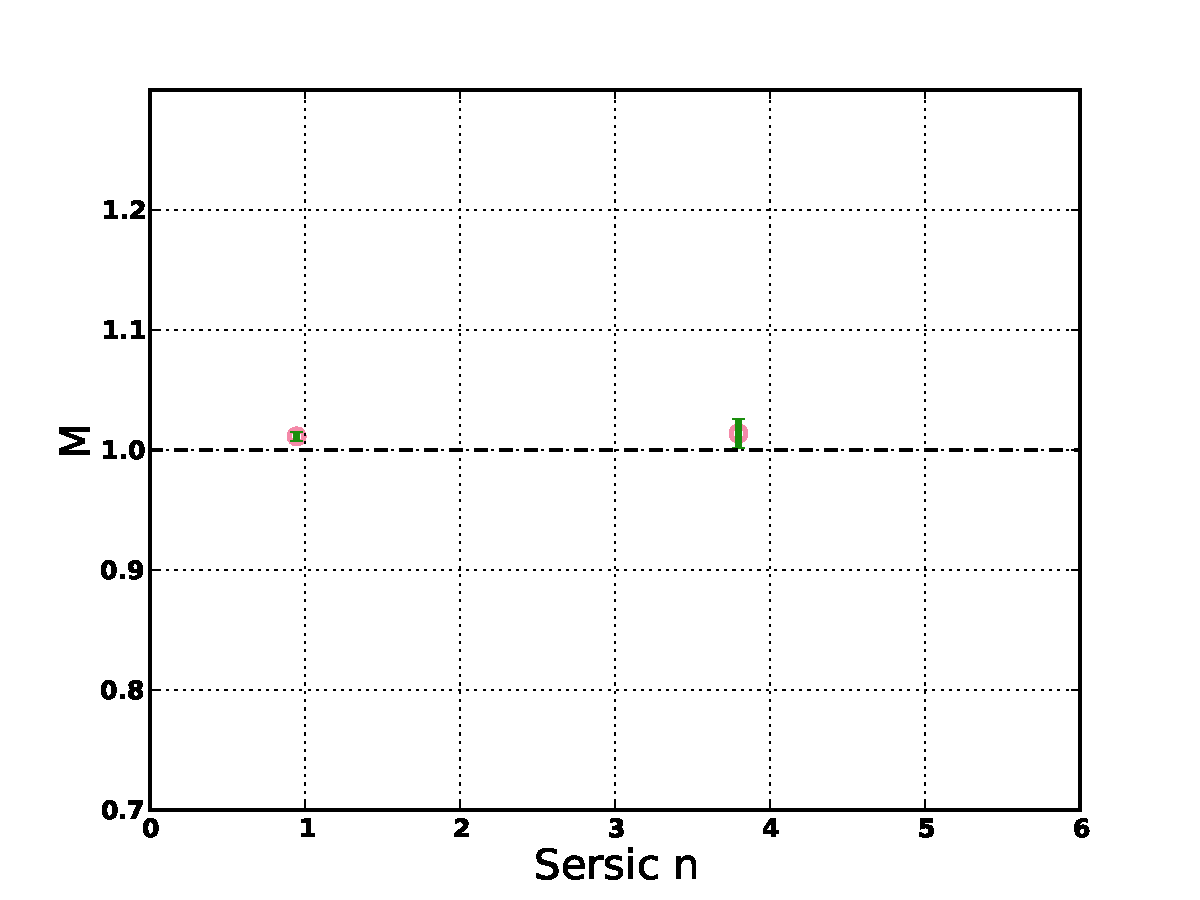
\includegraphics[width=0.45\textwidth]{fig/Mval_typeGM.pdf} 
%\includegraphics[width=0.45\textwidth]{fig/Mval_sizeGM.pdf} 
\caption{The M and C values for ...}
\label{fig:DEIMOS_m}
\end{figure*}

\newpage 
\subsection{im3shape}
im3shape is a modular shape measurement code that performs a maximum likelihood (ML) fit of a de Vaucouleurs bulge plus Exponential disc galaxy model to noisy images, incorporating an applied PSF (see Zuntz et al 2013/in prep.).  The software is written primarily in C with supporting Python infrastructure, and is publicly available.  For the ClusterSTEP data the PSF is modelled as an elliptical Moffat profile (1969), assumed to be constant across each chip.  Moffat profiles were fit (using the Levenberg-Marquardt algorithm) to stellar images in the ClusterSTEP data, and the chipwise model estimated from these individual fits using an inverse variance weighted average of the resulting best-fitting parameters. For the subset of fields in which the PSF was known to be Gaussian, a $\beta$ slope parameter of 1000 was fixed in the profile fitting process (the Moffat approaches the Gaussian profile for large $\beta$).

For galaxy shape measurement using parametric profiles, ML estimators are known to be biased due to the presence of noise (e.g., Refregier et al 2012; Kacprzak et al 2012).  For the tests in this paper a suite of noise bias-calibrating simulations were not conducted, due to resource constraints and the challenge of producing a representative calibration suite for data with realistic distributions of size and signal-to-noise such as ClusterSTEP:  the noise calibration schemes presented by Kacprzak et al (2012) and Zuntz et al (2013) were for far simpler distributions of galaxy properties.  Understanding how to build such suites is an active field of research, and of great relevance to the many methods with known noise bias issues.

The performance of im3shape shear estimates is therefore expected to degrade somewhat as signal-to-noise decreases.  Objects with an im3shape-determined signal-to-noise (in total flux) of lower than 10 were excluded in the final catalogue, along with catastrophic outliers in the value of the best likelihood, and objects for which any pixel value in a model-minus-data residual image was found to be greater than the peak pixel flux in the data.
\begin{figure*}
\centering
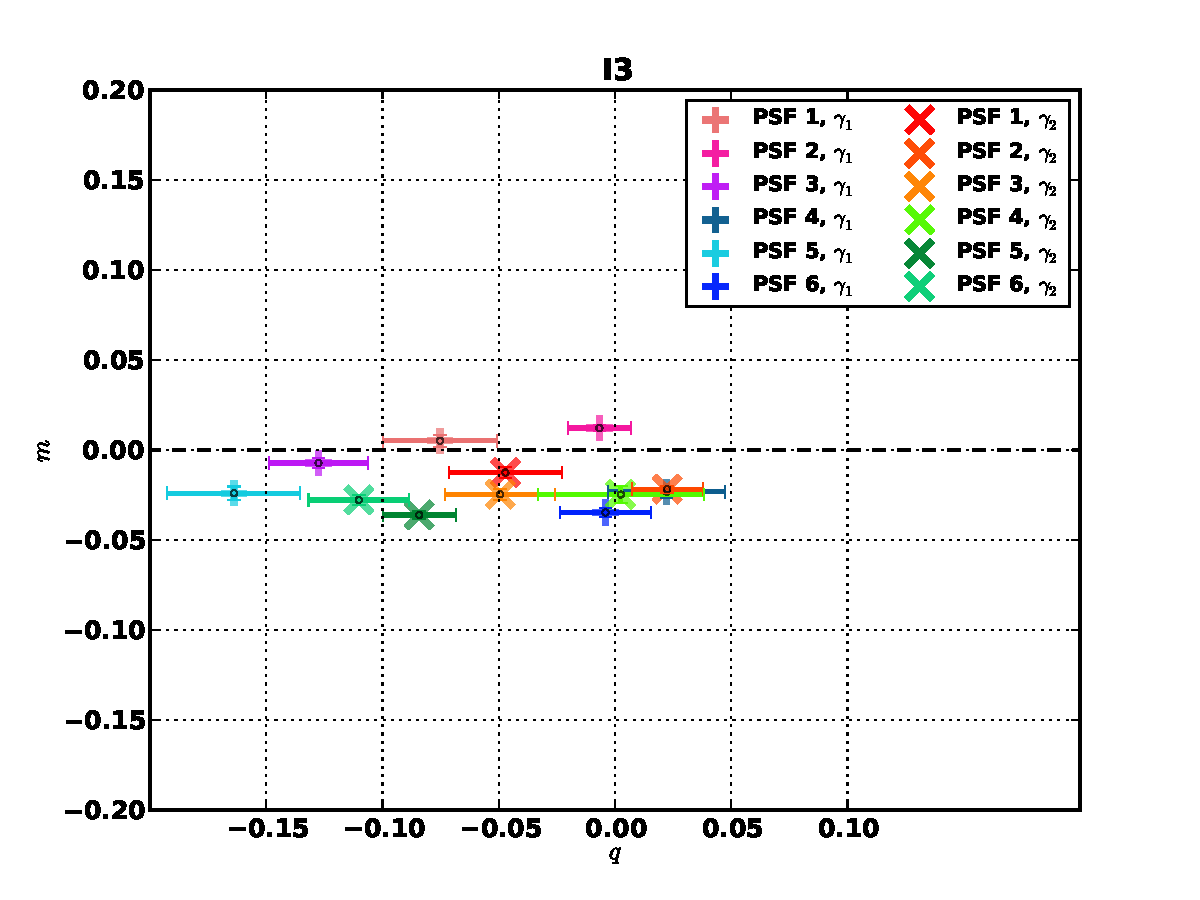
\includegraphics[width=0.45\textwidth]{fig/QMC_main_I3_f.pdf} 
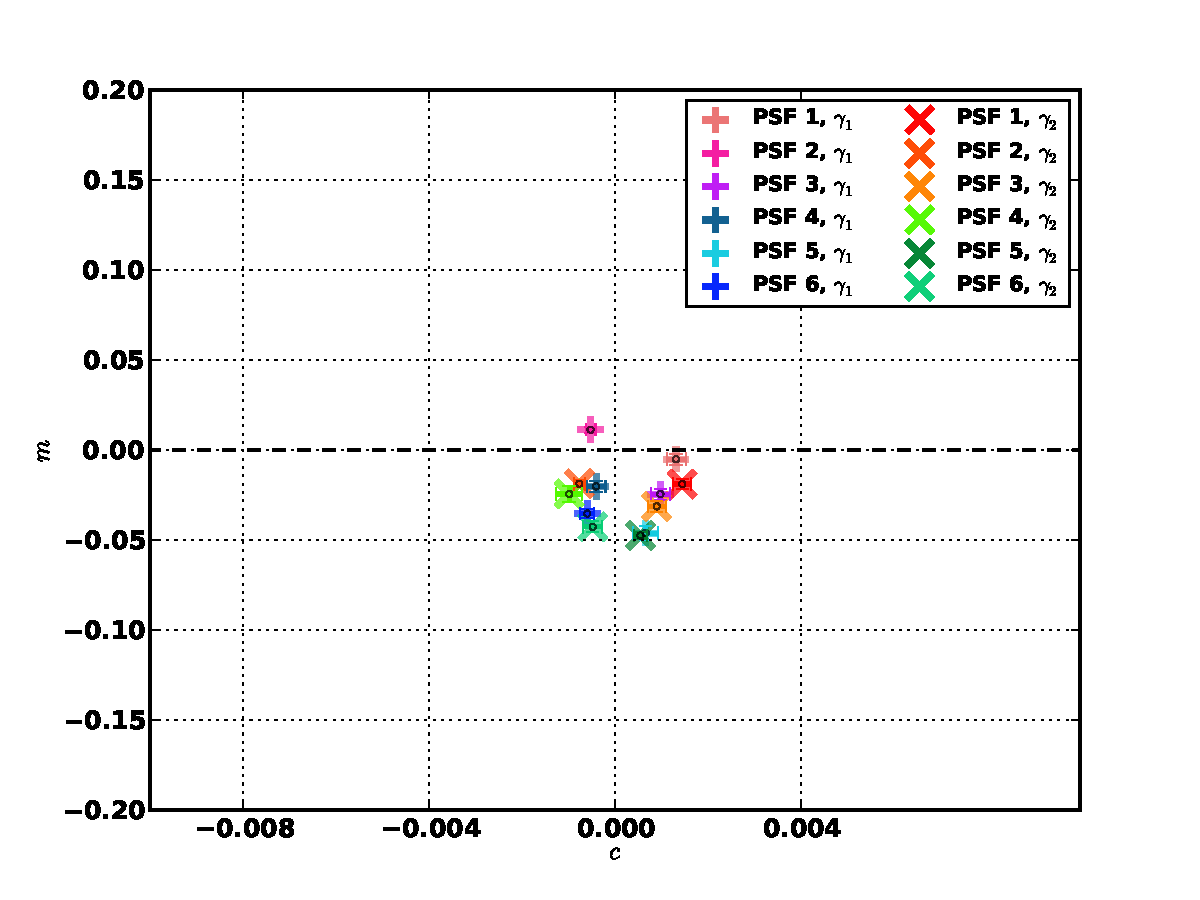
\includegraphics[width=0.45\textwidth]{fig/MC_main_I3_f.pdf} 
\caption{Average Q and M results for all pipelines for objects 
SNR $>$ 20 on the left and M and C results for all pipelines for objects 
SNR $>$ 20 on the right seperate by $\gamma_{1} $ and $\gamma_{2} $ as
well as PSF.}
\label{fig:im3shape_qmc}
\end{figure*}

\begin{figure*}
\centering
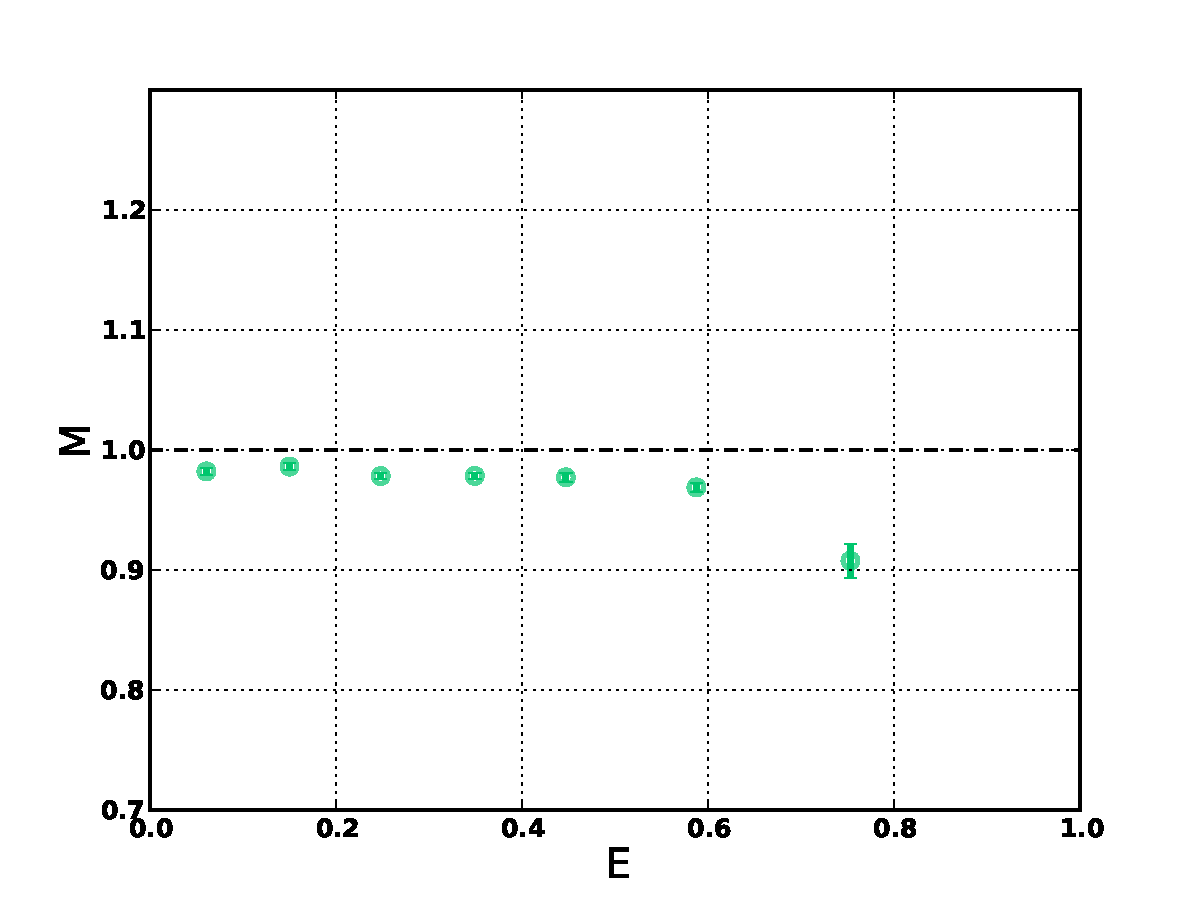
\includegraphics[width=0.45\textwidth]{fig/MvaleI3.pdf} 
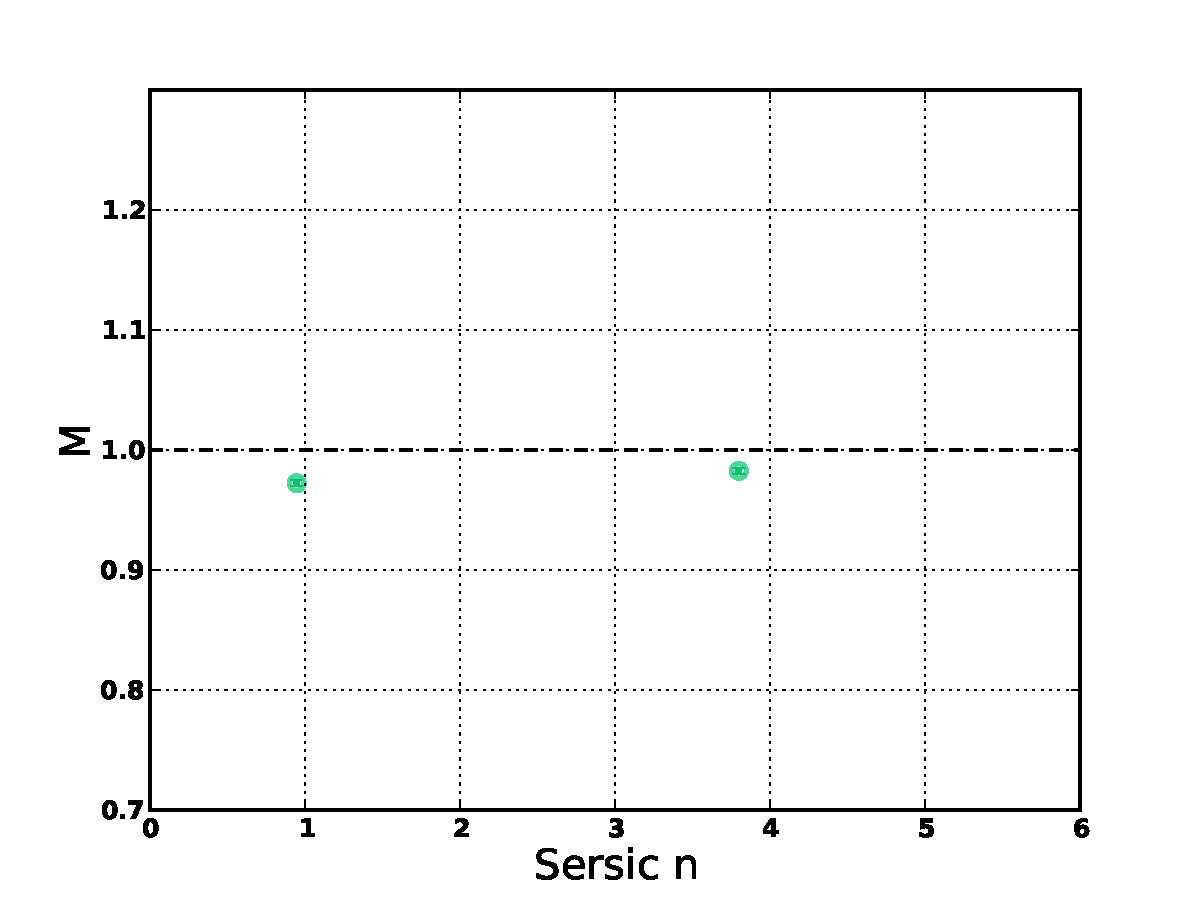
\includegraphics[width=0.45\textwidth]{fig/Mval_typeI3.pdf} 
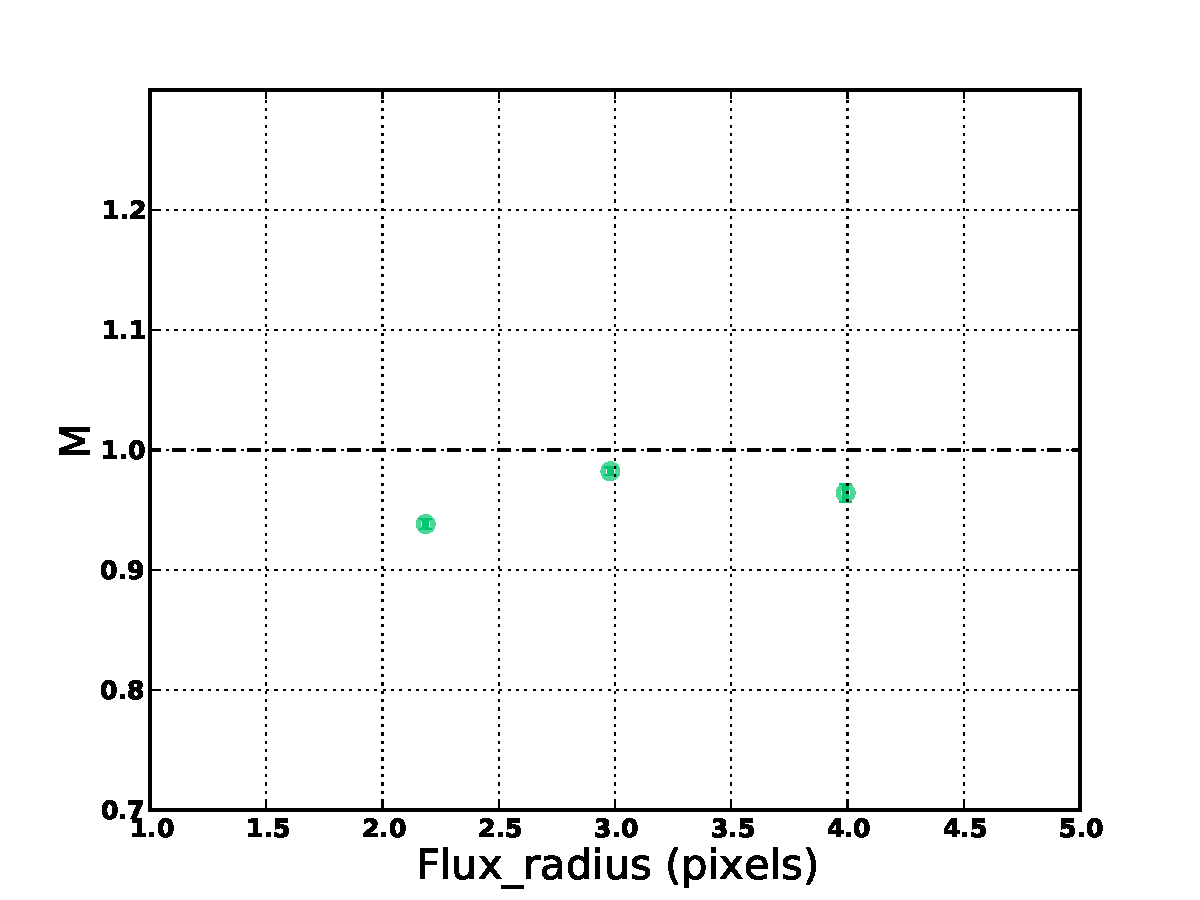
\includegraphics[width=0.45\textwidth]{fig/Mval_sizeI3.pdf} 
\caption{The M and C values for ...}
\label{fig:DEIMOS_m}
\end{figure*}

\newpage 
\subsection{BJ02}
\begin{figure*}
\centering
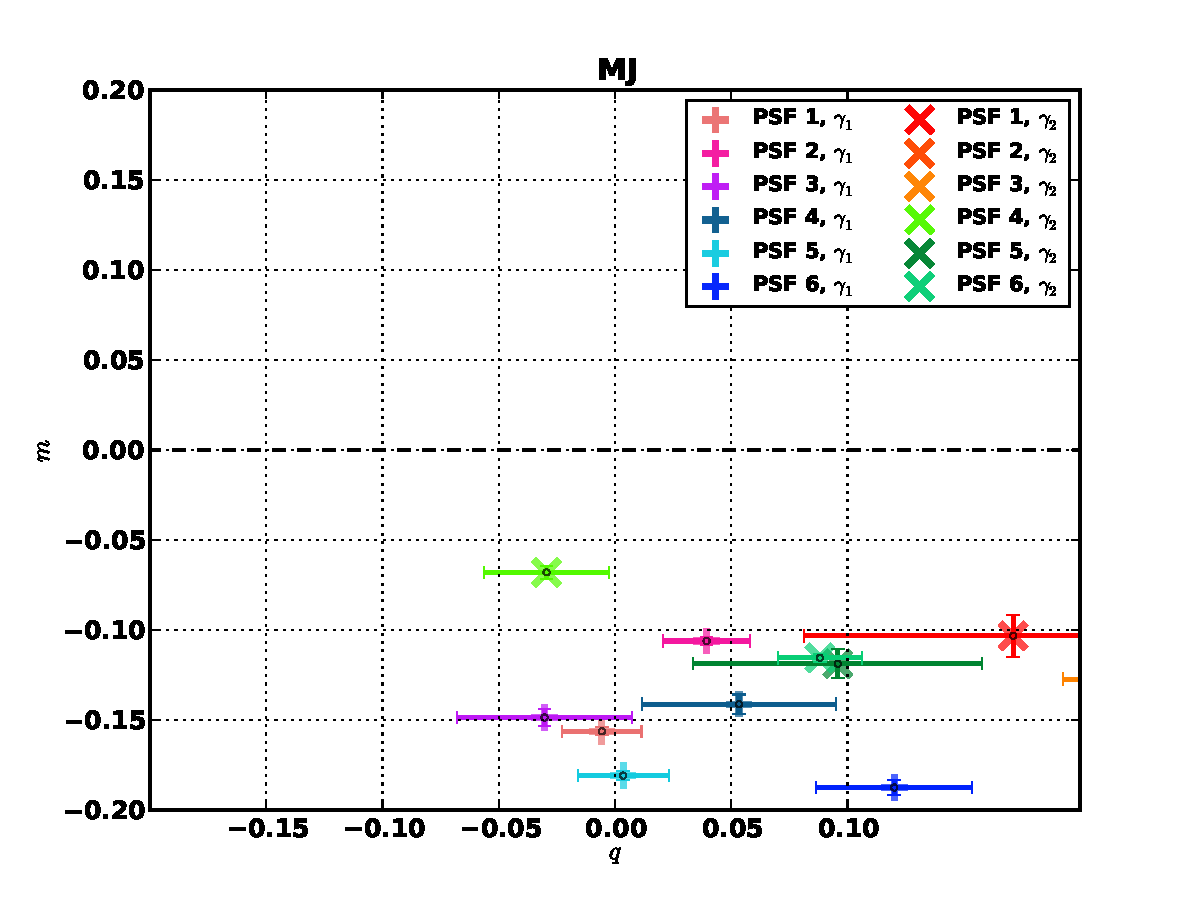
\includegraphics[width=0.45\textwidth]{fig/QMC_main_MJ_f.pdf} 
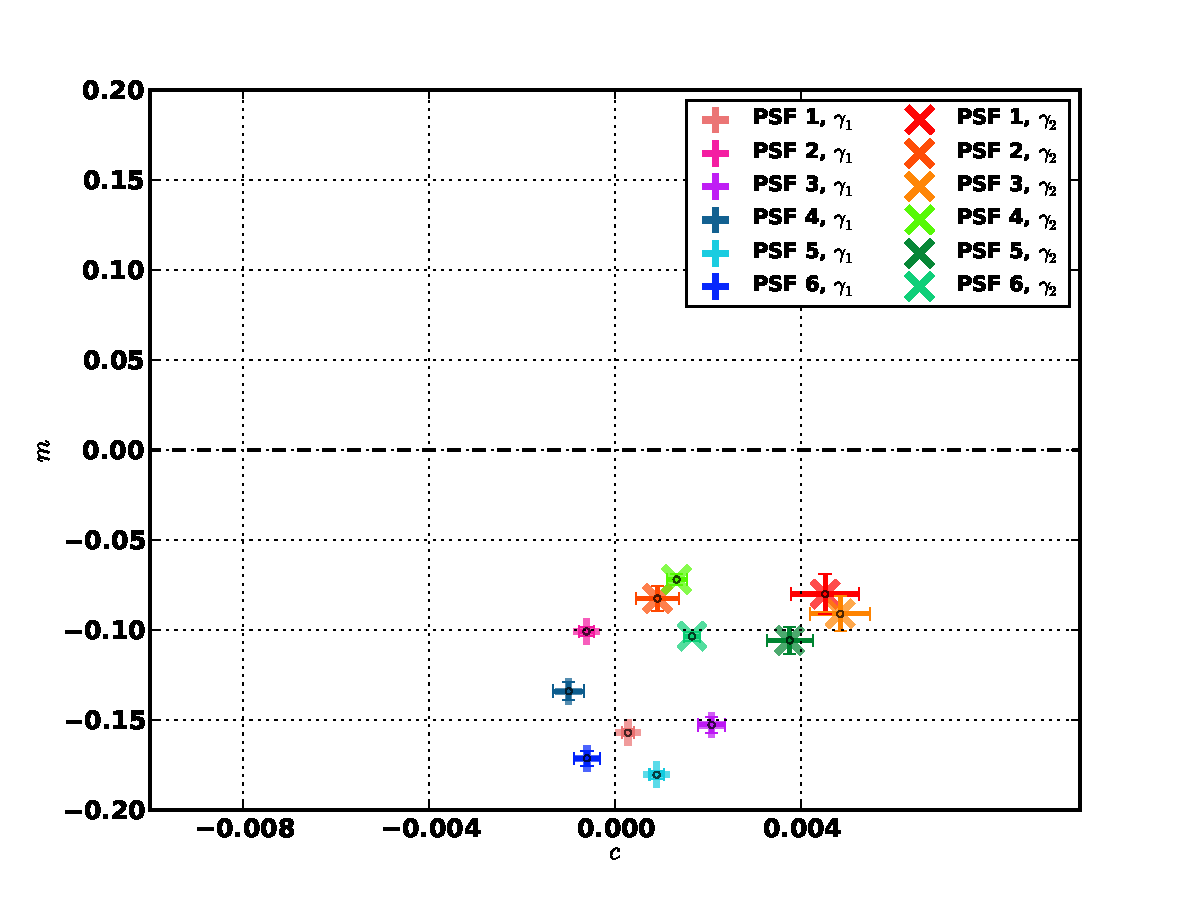
\includegraphics[width=0.45\textwidth]{fig/MC_main_MJ_f.pdf} 
\caption{Average Q and M results for all pipelines for objects 
SNR $>$ 20 on the left and M and C results for all pipelines for objects 
SNR $>$ 20 on the right seperate by $\gamma_{1} $ and $\gamma_{2} $ as
well as PSF.}
\label{fig:BJ_qmc}
\end{figure*}

\begin{figure*}
\centering
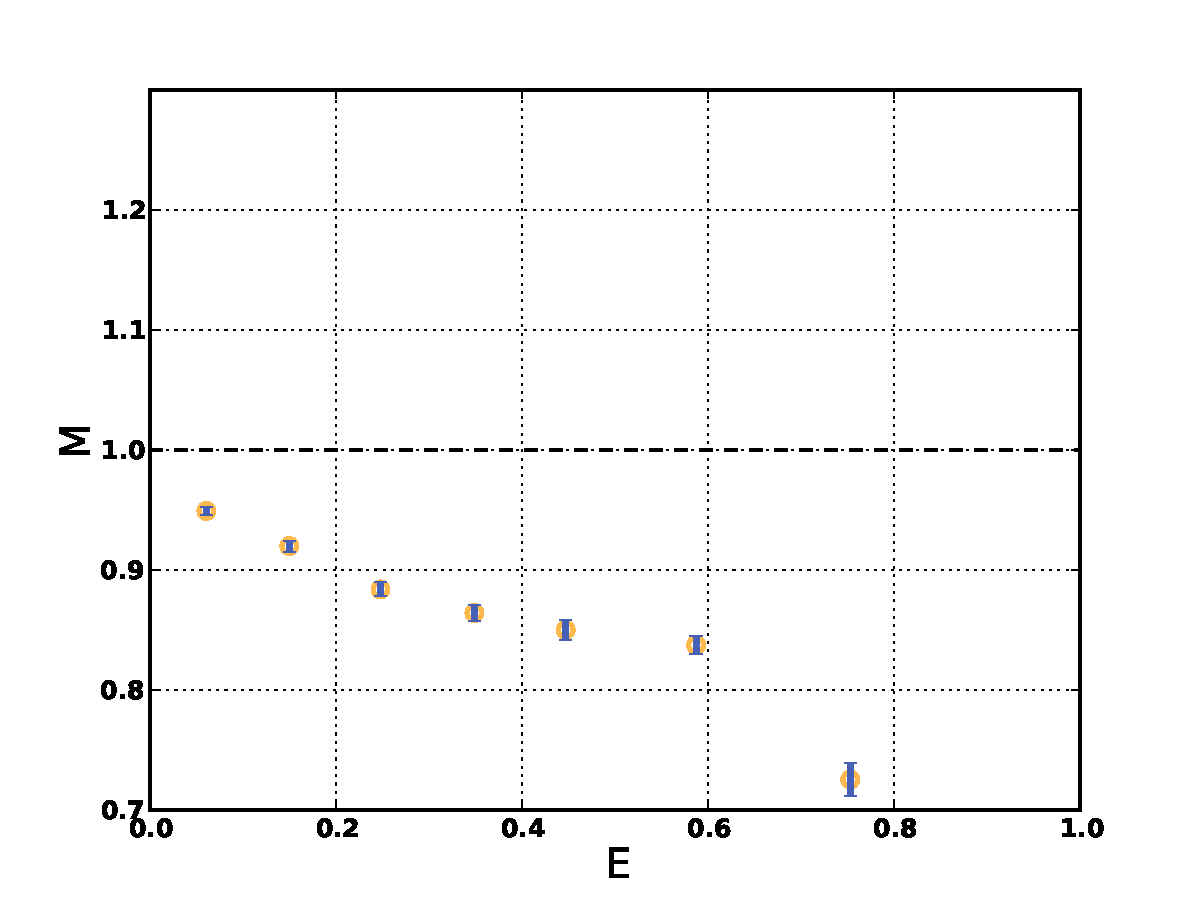
\includegraphics[width=0.45\textwidth]{fig/MvaleMJ.pdf} 
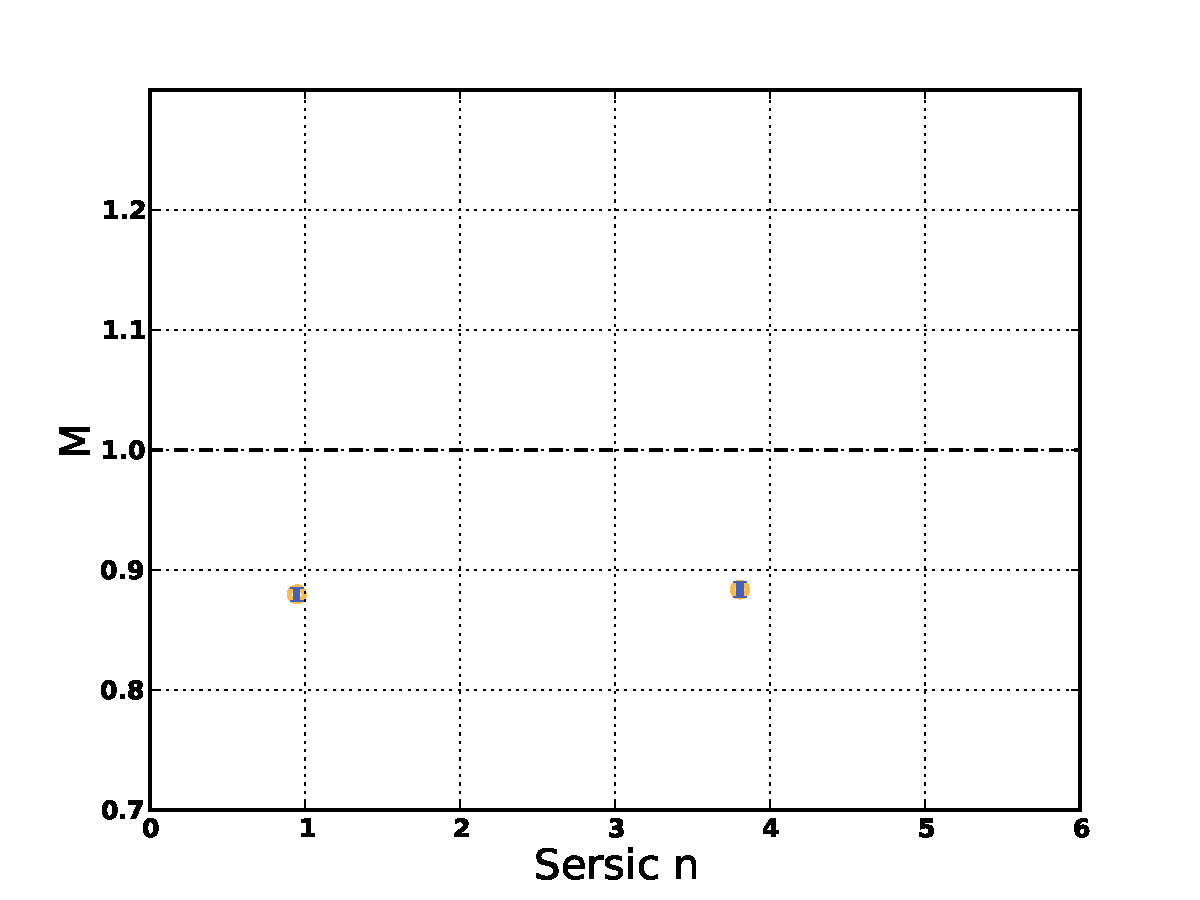
\includegraphics[width=0.45\textwidth]{fig/Mval_typeMJ.pdf} 
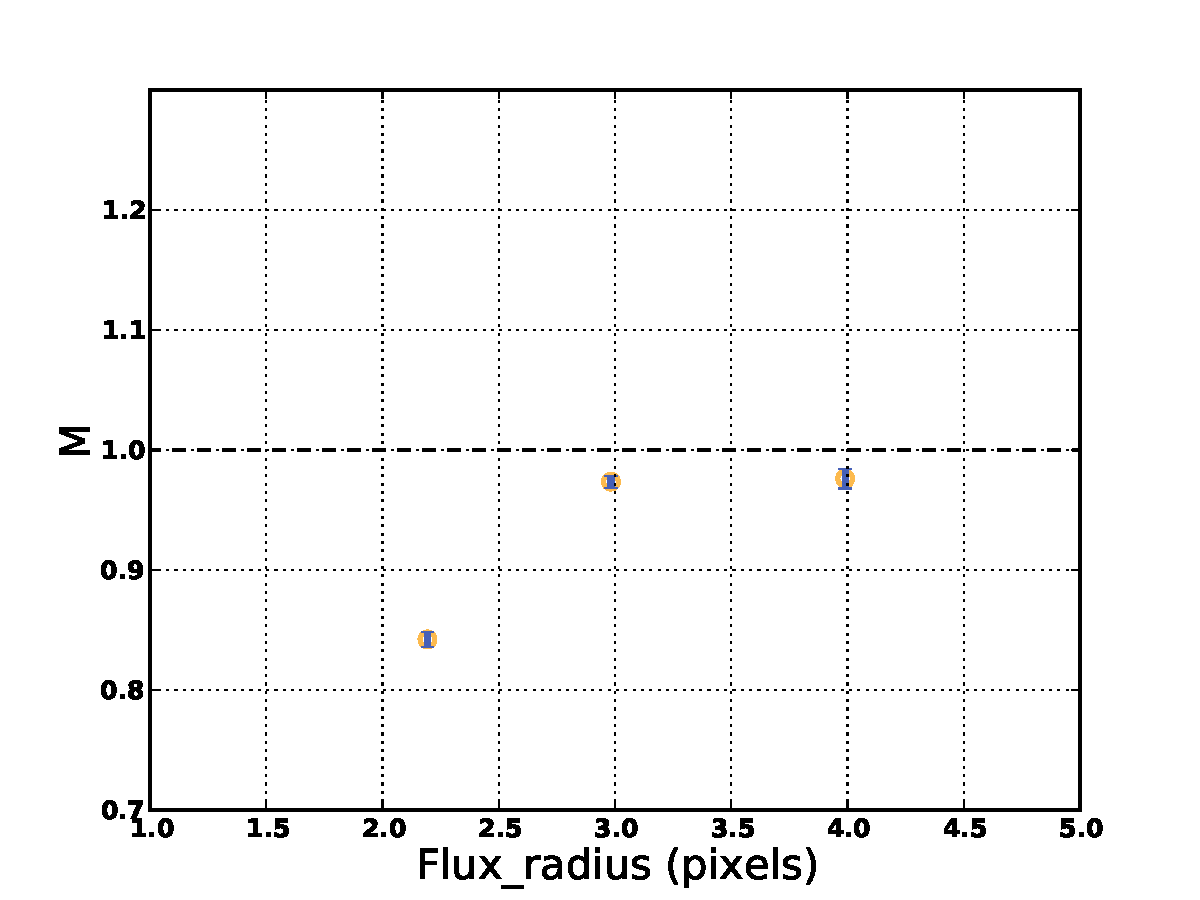
\includegraphics[width=0.45\textwidth]{fig/Mval_sizeMJ.pdf} 
\caption{The M and C values for ...}
\label{fig:DEIMOS_m}
\end{figure*}

\newpage 
\subsection{PFDNT}
For PFDNT we prepare time image postage stamp and PSF model in the
same way. Shear is estimated by applying roundness tests on the
anti-sheared, deconvolved Fourier transform of the image. To this end,
we use a weight function limited to frequencies where the Fourier
transform of the PSF is above zero according to Bernstein (2010). We
use the ellipticity estimate from the PKSB pipeline as a starting
point and sample ellipticities on a hexagonal grid to find the shear
estimate as the probability-weighted integral over ellipticity
space. \\

\begin{figure*}
\centering
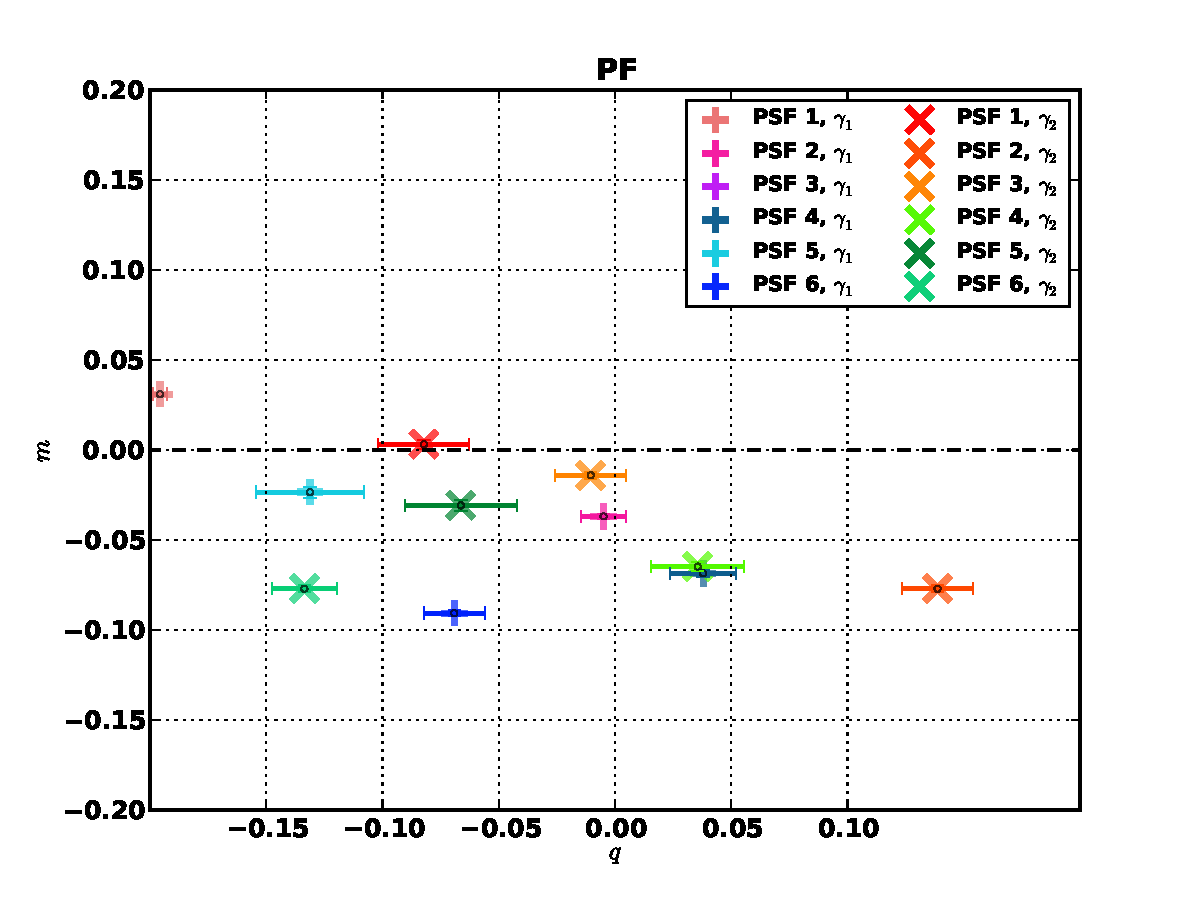
\includegraphics[width=0.45\textwidth]{fig/QMC_main_PF_f.pdf} 
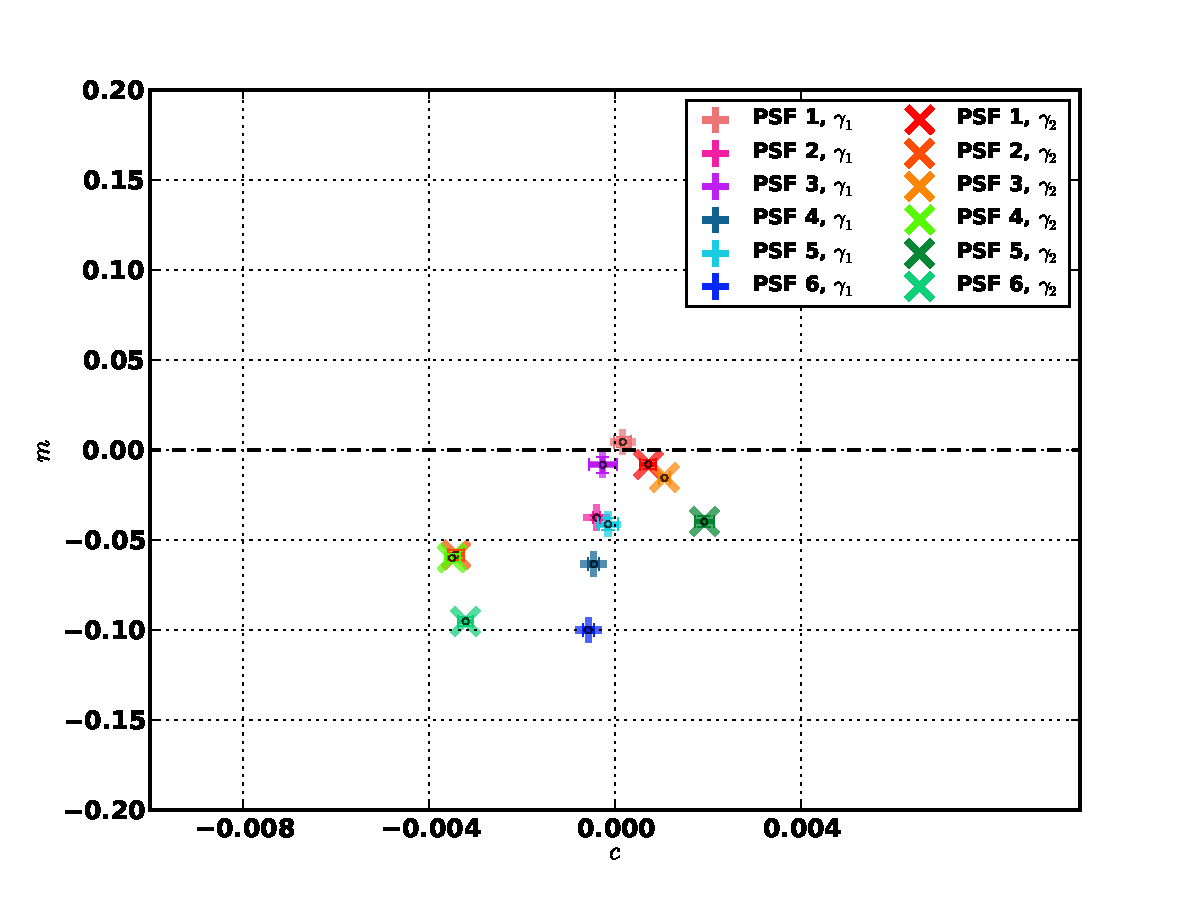
\includegraphics[width=0.45\textwidth]{fig/MC_main_PF_f.pdf} 
\caption{Average Q and M results for all pipelines for objects 
SNR $>$ 20 on the left and M and C results for all pipelines for objects 
SNR $>$ 20 on the right seperate by $\gamma_{1} $ and $\gamma_{2} $ as
well as PSF.}
\label{fig:PFDNT_qmc}
\end{figure*}
\begin{figure*}
\centering
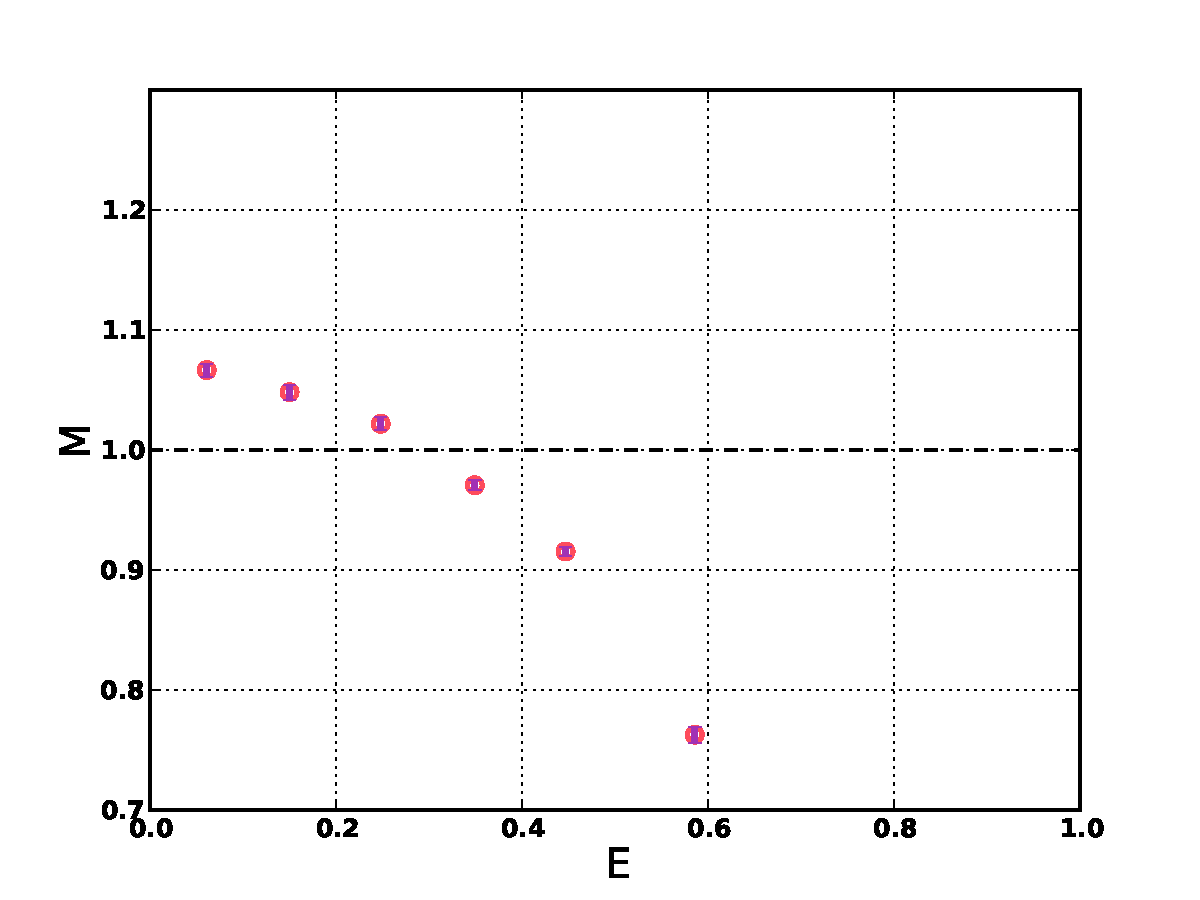
\includegraphics[width=0.45\textwidth]{fig/MvalePF.pdf} 
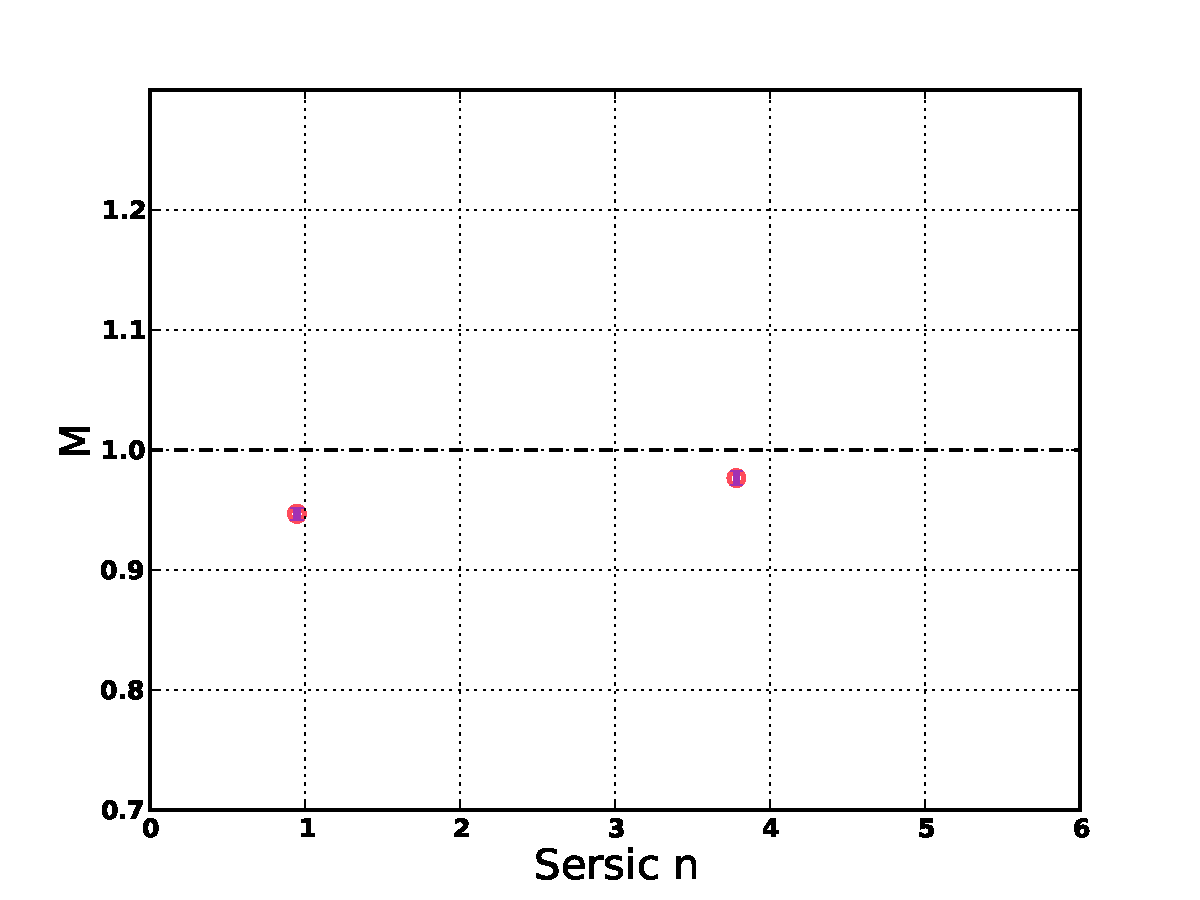
\includegraphics[width=0.45\textwidth]{fig/Mval_typePF.pdf} 
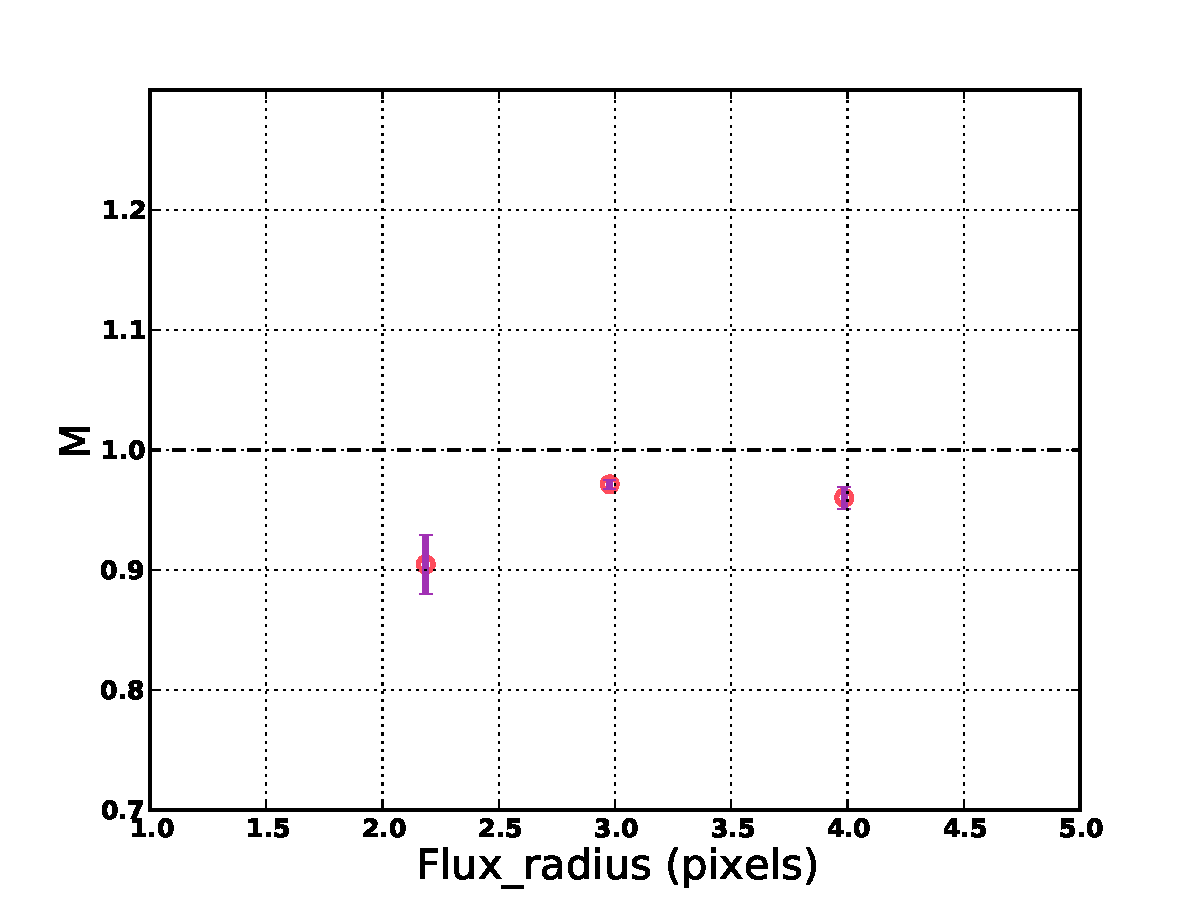
\includegraphics[width=0.45\textwidth]{fig/Mval_sizePF.pdf} 
\caption{The M and C values for ...}
\label{fig:DEIMOS_m}
\end{figure*}

\clearpage